\secnumbersection{VALIDACIÓN DE LA SOLUCIÓN}

Esta sección valida empíricamente DRAFTS++ mediante casos de uso que demuestran funcionalidad, robustez temporal y escalabilidad, además de evaluar estrategias de detección en alta frecuencia (86 GHz).

% La metodología de validación implementada sigue un enfoque sistemático y comparativo que garantiza la reproducibilidad de los resultados. Para cada componente, se establecieron métricas de evaluación específicas, se utilizaron datasets de referencia validados por la literatura científica, y se implementaron protocolos de verificación independientes con grupos de astrónomos colaboradores.

% Los objetivos principales de esta validación incluyen: (1) demostrar la superioridad de los pipelines desarrollados respecto a métodos existentes, (2) validar la capacidad de procesamiento de archivos de gran tamaño, (3) confirmar la precisión temporal y espacial en la detección de eventos, (4) evaluar la eficiencia computacional y escalabilidad del sistema, y (5) establecer la capacidad de descubrimiento científico mediante la detección de eventos nuevos no reportados previamente en la literatura.

\subsection{VALIDACIÓN DEL COMPONENTE 1: DRAFTS++ - Pipeline astronómico E2E, Productivo, Robusto y Eficiente}

La validación utiliza tres casos progresivos que ejercitan las siete etapas del pipeline (Figura~\ref{fig:workflow-src}) bajo complejidad creciente:

\begin{enumerate}
    \item \textbf{FAST-FREX (Radiotelescopio FAST)}: Dataset de entrenamiento del Five-hundred-meter Aperture Spherical Telescope (FAST, China) que valida flujo completo E2E con modelos CenterNet/ResNet18 integrados. Formato PSRFITS, frecuencia central $\sim$1.25 GHz.
    
    \item \textbf{Pulsar B0355+54 (Radiotelescopio FAST)}: Observación de 117s del radiotelescopio FAST conteniendo 752 pulsos teóricos del púlsar B0355+54 (periodo 0.156s) que valida streaming, continuidad temporal y trazabilidad (732/752 detectados, 97.3\%). Formato PSRFITS.
    
    \item \textbf{FRB 121102 (Radiotelescopio Effelsberg)}: 6 archivos de observación del radiotelescopio Effelsberg de 100m (Alemania) en banda L ($\sim$1.4 GHz), cada uno de $\sim$4 GB, que validan escalabilidad, gestión de memoria y descubrimiento científico (Recall 100\%, 2 nuevos bursts). Datos reportados por \cite{cruces2020frb121102}.
\end{enumerate}

El éxito en los tres casos demuestra que todas las etapas del pipeline operan coordinadamente. Cualquier falla en etapas principales o módulos de soporte causaría fallos completos del sistema.

\begin{table}[H]
\centering
\caption{Mapeo entre etapas del pipeline DRAFTS++ y casos de validación implementados. Cada caso ejercita múltiples etapas de manera integrada, demostrando cobertura completa del sistema mediante validación E2E.}
\label{tab:mapeo_validacion_etapas_componente1}
\small
\begin{tabular}{|l|c|c|c|}
\hline
\textbf{Etapa del Pipeline} & \textbf{Caso 1} & \textbf{Caso 2} & \textbf{Caso 3} \\
\textbf{(Figura~\ref{fig:workflow-src})} & \textbf{FAST-FREX} & \textbf{B0355+54} & \textbf{FRB121102} \\
\hline
\texttt{input/} Ingesta & \checkmark & \checkmark & \textbf{Masivo} \\
\texttt{preprocessing/} Preprocesamiento & Básico & \textbf{Streaming} & \textbf{Chunking} \\
\texttt{models/} Modelos & \checkmark & \checkmark & \checkmark \\
\texttt{detection/} Detección & \checkmark & \textbf{732 pulsos} & \textbf{Recall 100\%} \\
\texttt{analysis/} Análisis & \checkmark & \textbf{Temporal} & \textbf{Física} \\
\texttt{visualization/} Visualización & \checkmark & \checkmark & \checkmark \\
\texttt{output/} Artefactos & \checkmark & \checkmark & \checkmark \\
\hline
\texttt{core/} Orquestación & Implícito & Implícito & \textbf{Memoria} \\
\texttt{config/} Configuración & \checkmark & \checkmark & \checkmark \\
\texttt{logging/} Registro & \checkmark & \checkmark & \checkmark \\
\texttt{scripts/} CLI & \checkmark & \checkmark & \checkmark \\
\hline
\textbf{Foco de Validación} & Funcionalidad & Robustez & Escalabilidad \\
 & básica E2E & temporal & + Descubrimiento \\
\hline
\end{tabular}
\end{table}

\noindent\textbf{Leyenda:} \checkmark = Validado implícitamente; Básico = Configuración simple; \textbf{Énfasis} = Validación explícita crítica para el caso.

\subsubsection{Caso 1 - FAST-FREX: Validación Funcional Básica del Flujo E2E}

FAST-FREX es el dataset de entrenamiento del pipeline DRAFTS original, adquirido con el radiotelescopio FAST (Five-hundred-meter Aperture Spherical Telescope, China), el radiotelescopio de plato único más grande del mundo. Este caso valida el flujo completo E2E: ingesta multi-formato PSRFITS, análisis automático de headers, visualización científica y integración automatizada de modelos CenterNet/ResNet18. Las observaciones se realizaron en banda L ($\sim$1.25 GHz) con resolución temporal milisegundo.

\begin{figure}[H]
    \centering
    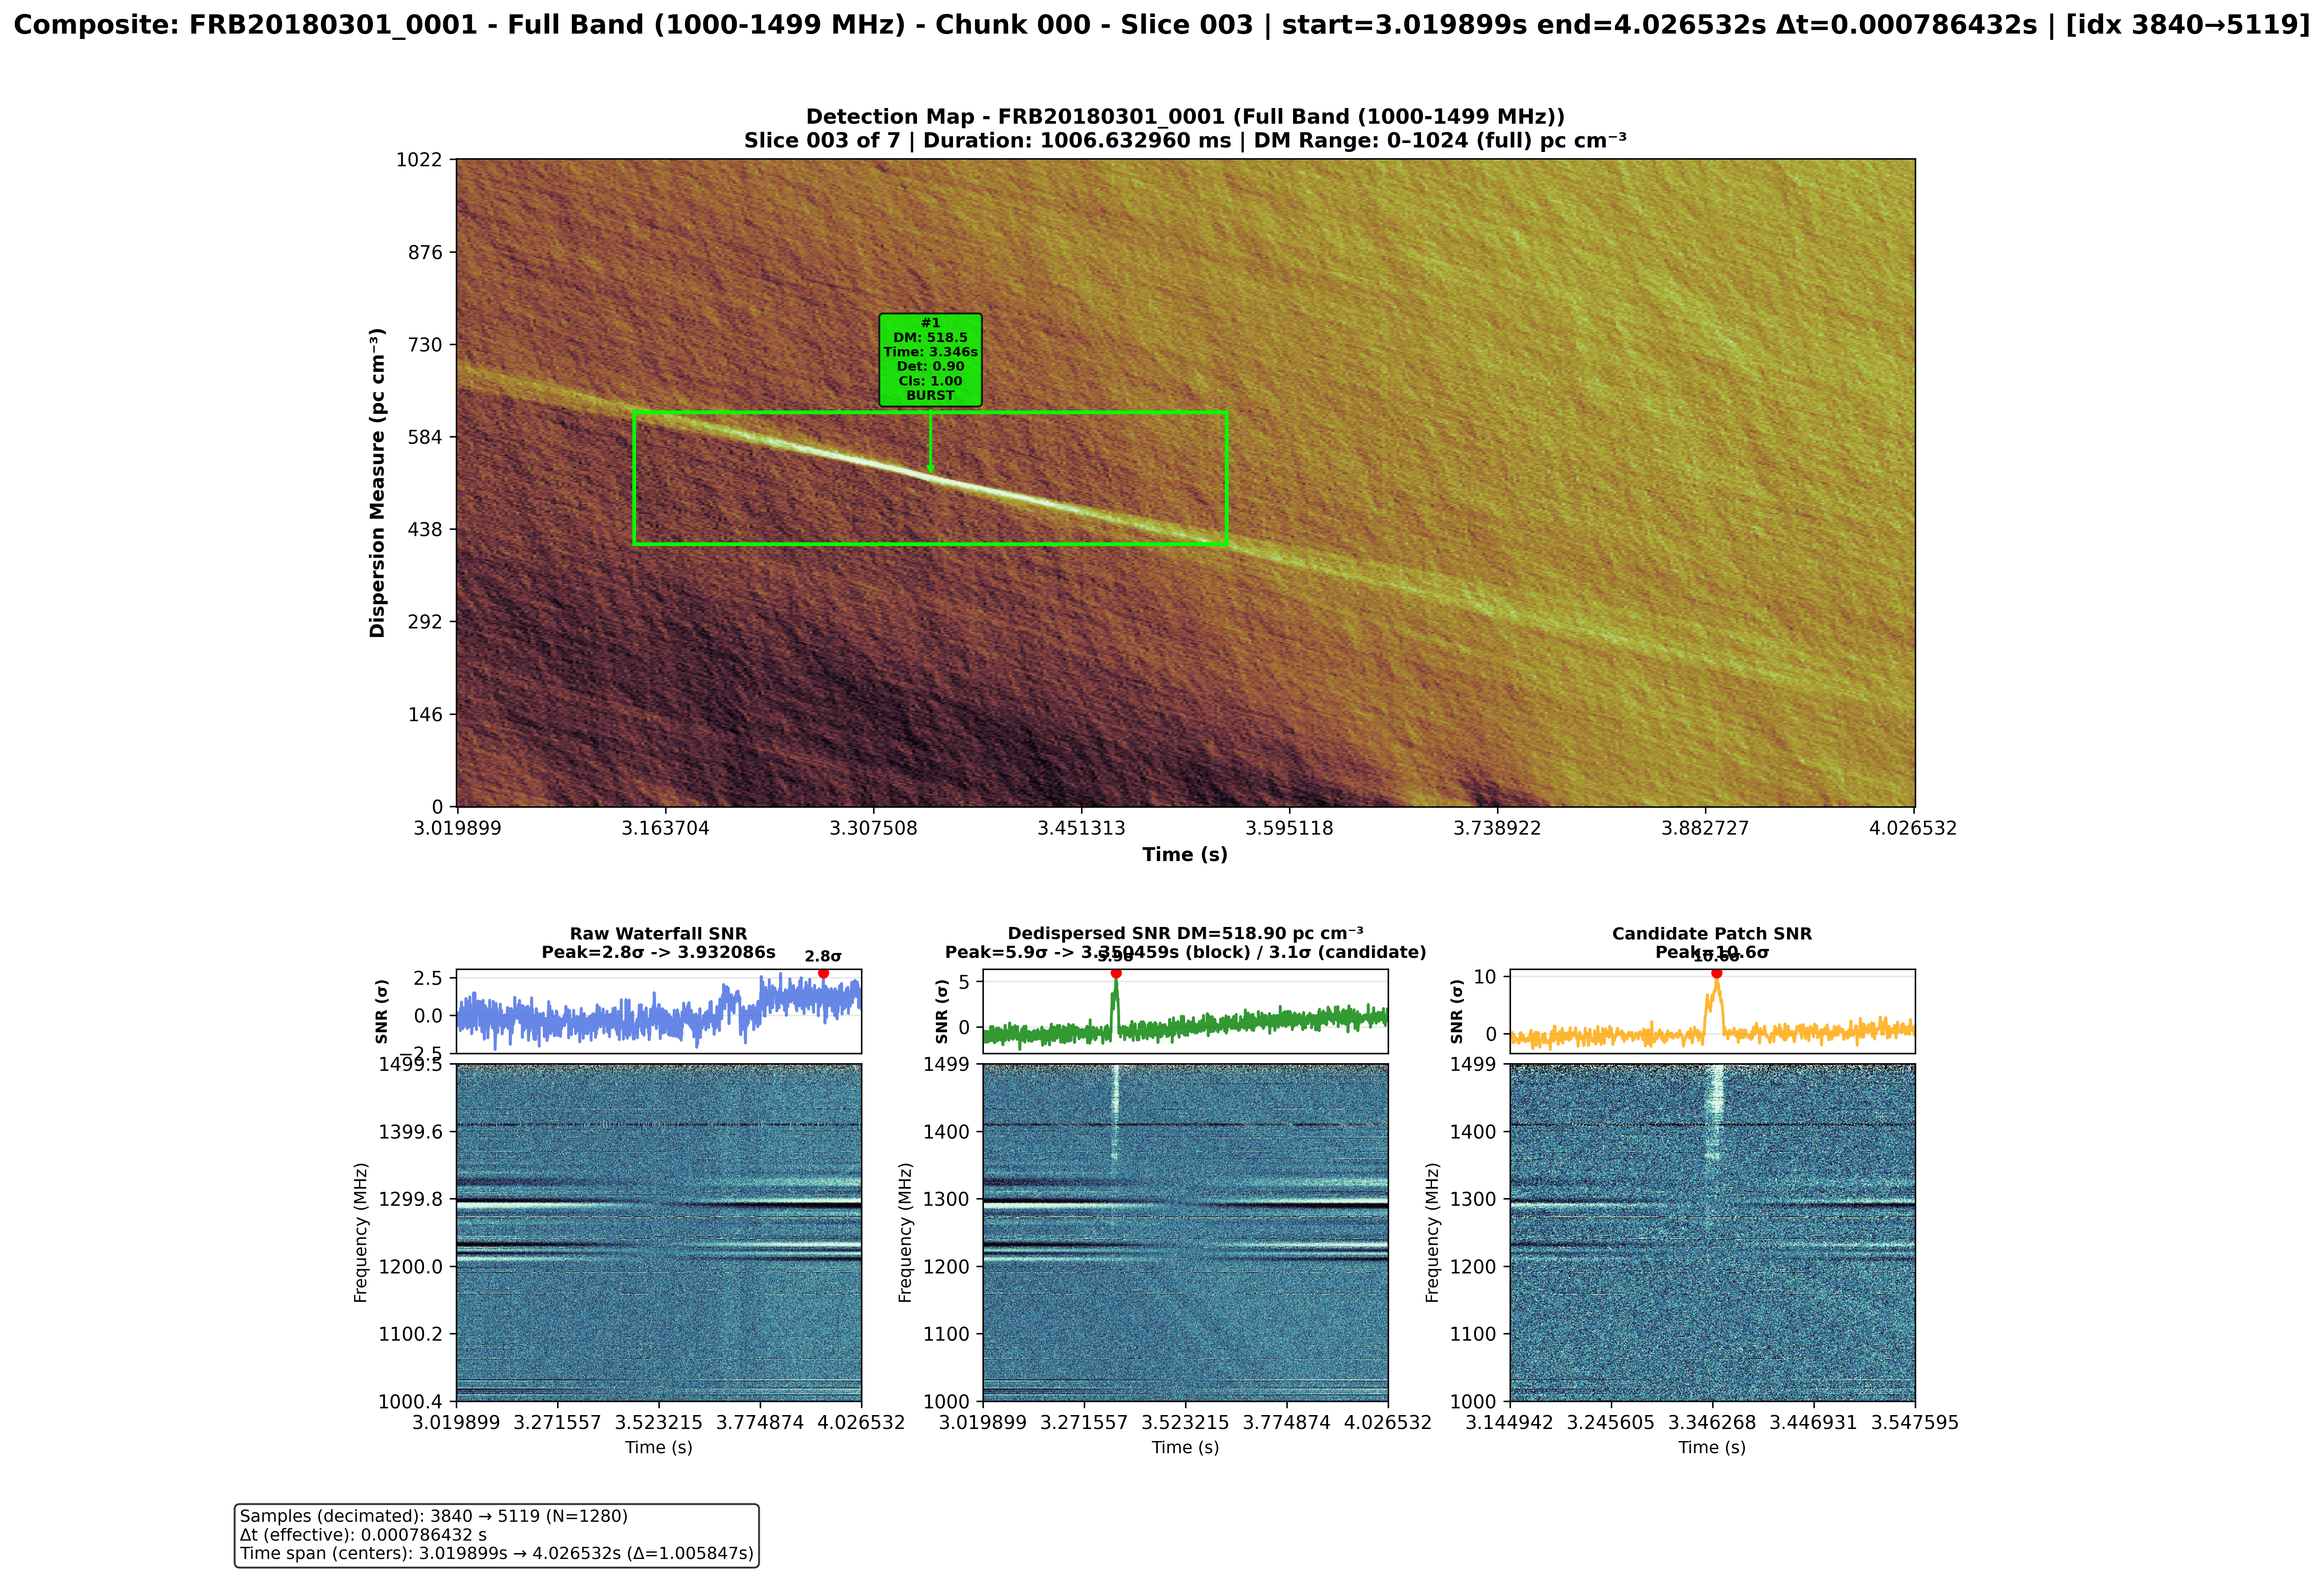
\includegraphics[width=\textwidth]{figures/FRB20180301_0001_slice003.png}
    \caption[Detección FRB (FAST-FREX)]{Detección FRB con SNR de 5.9$\sigma$ mostrando mapa DM-tiempo y perfiles SNR crudo/dedispersado.}
    \label{fig:frb20180301_0001_slice003}
\end{figure}

\begin{figure}[H]
    \centering
    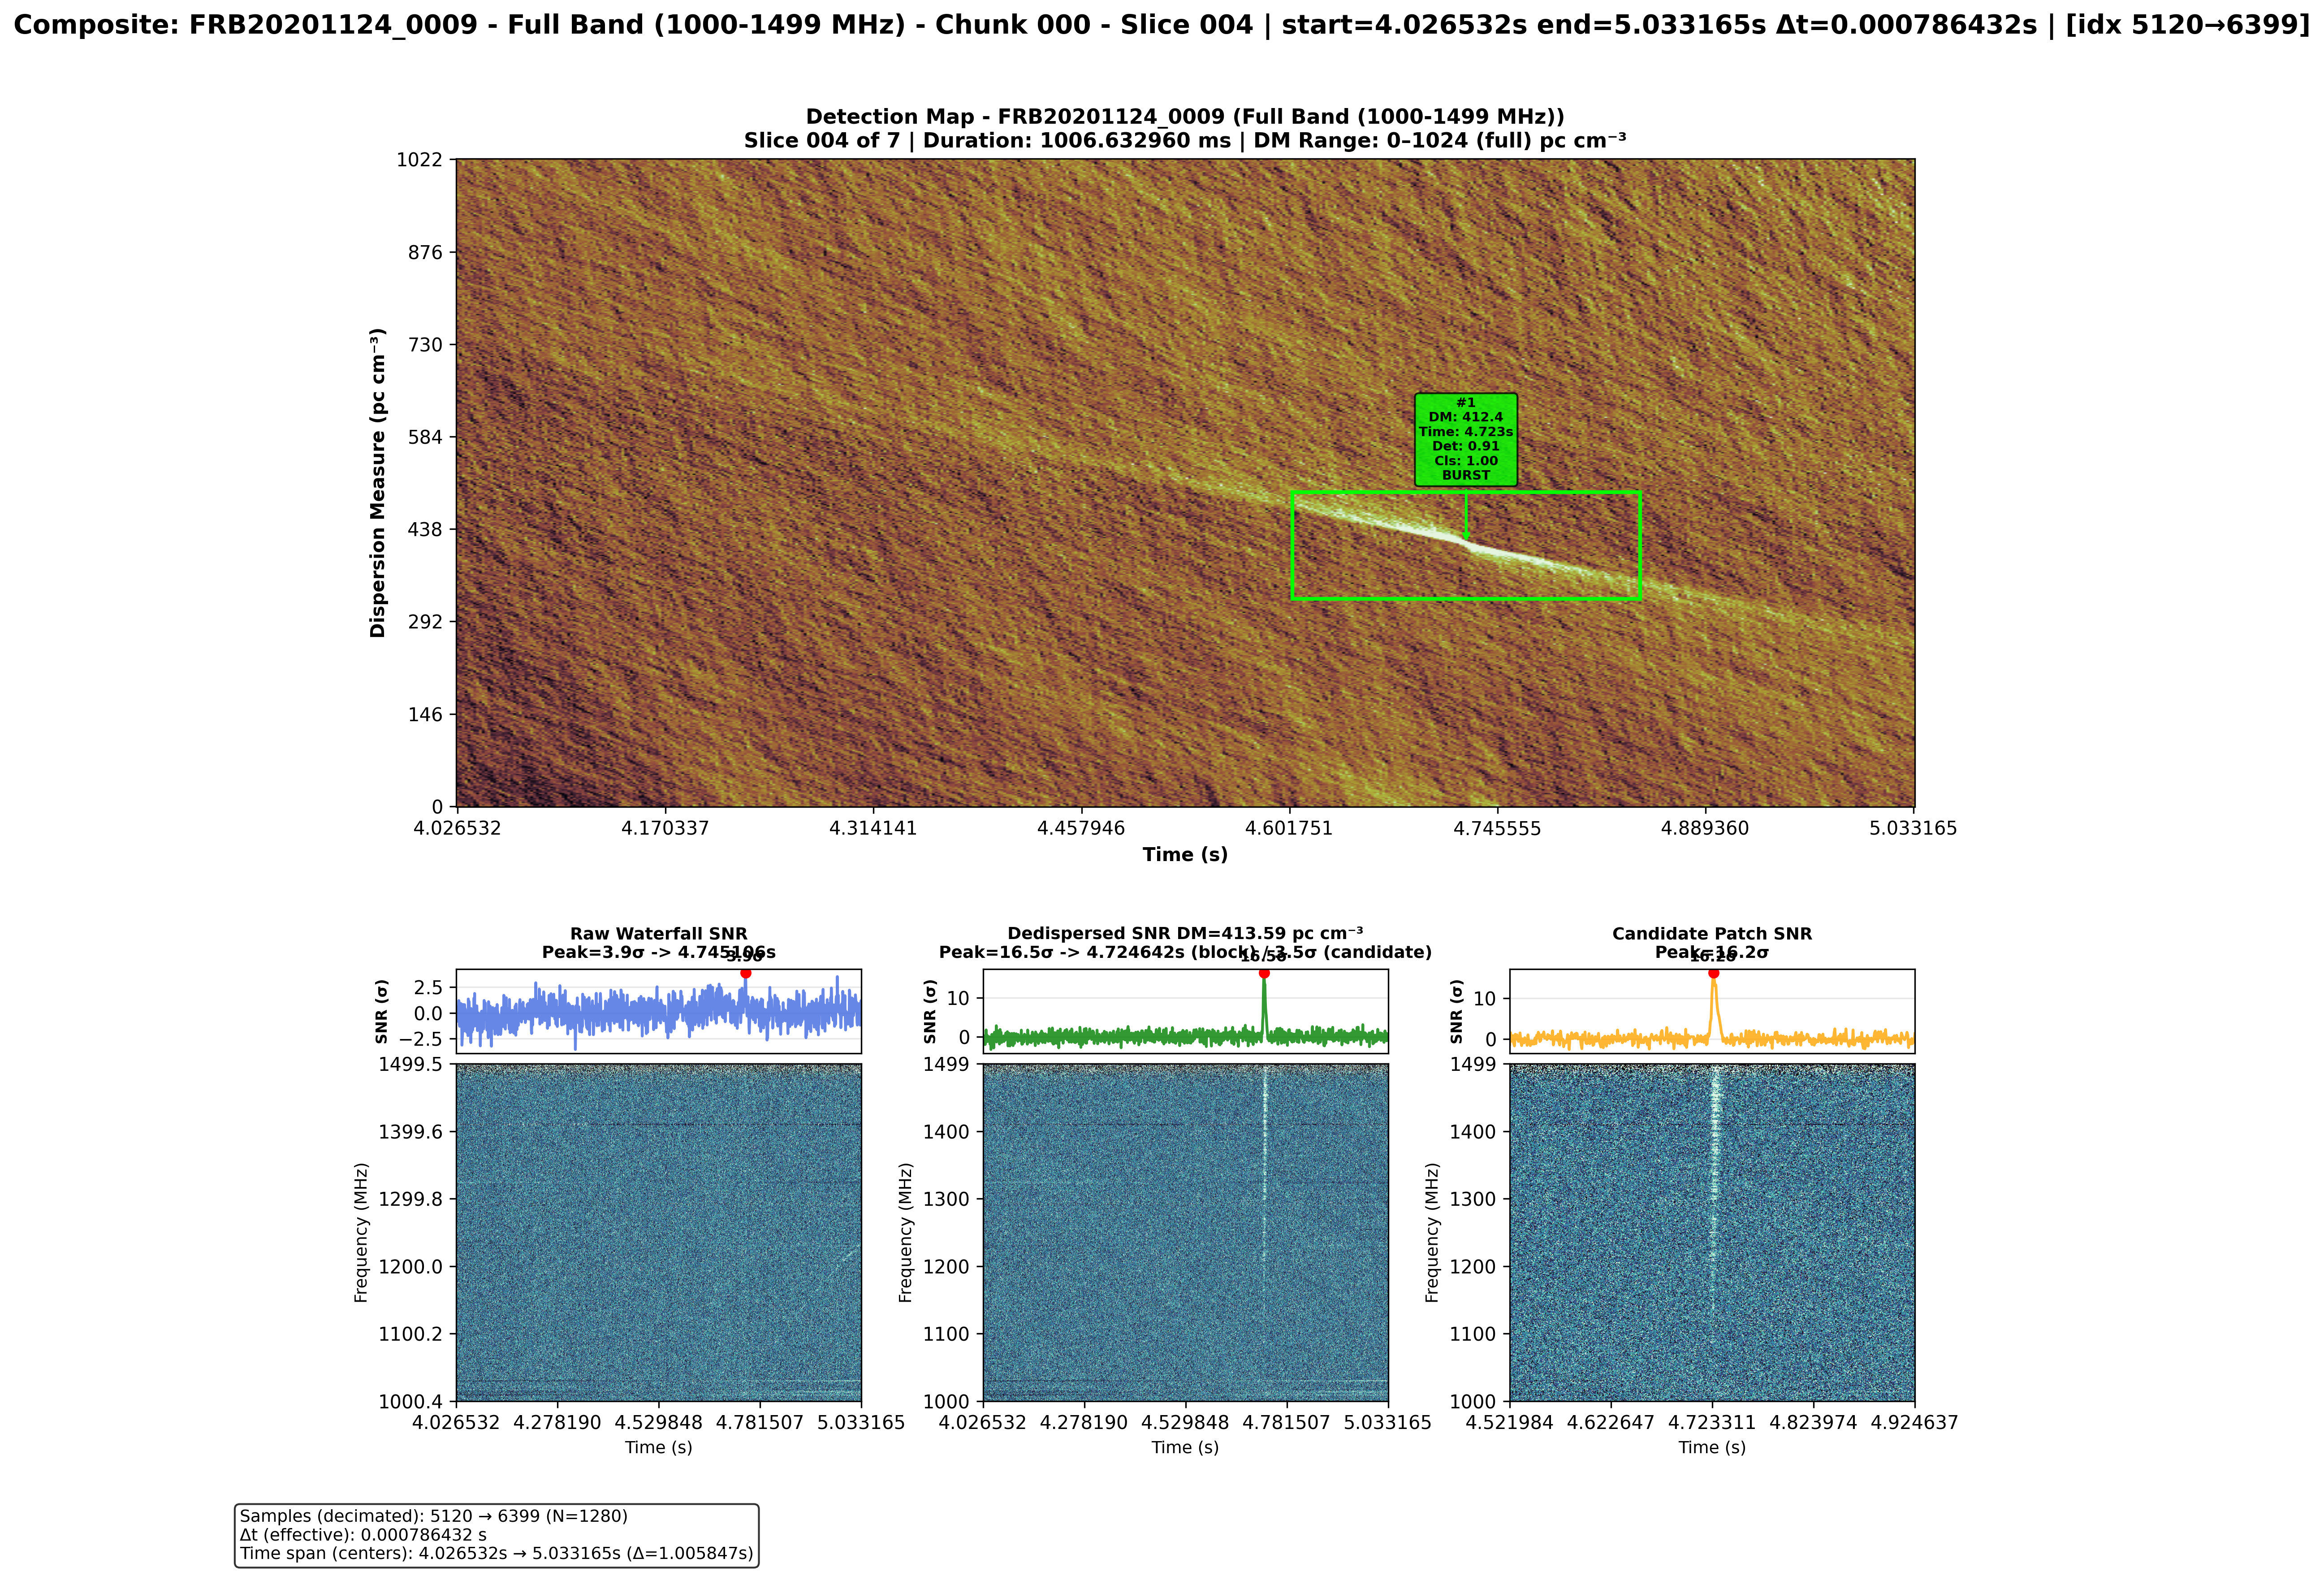
\includegraphics[width=\textwidth]{figures/FRB20201124_0009_slice004.png}
    \caption[Detección FRB adicional (FAST-FREX)]{Segundo FRB detectado con SNR de 16.5$\sigma$ confirmando efectividad del sistema.}
    \label{fig:frb20201124_0009_slice004}
\end{figure}

\subsubsection{Caso 2 - Pulsar B0355+54: Validación de Robustez Temporal y Procesamiento Secuencial}

Este caso utiliza observaciones del púlsar B0355+54 adquiridas con el radiotelescopio FAST en banda L ($\sim$1.25 GHz) en formato PSRFITS. El dataset valida mejoras de preprocesamiento: contigüidad temporal quirúrgica, streaming por slices, trazabilidad temporal precisa, manejo de discontinuidades y validación física integrada.

Características del dataset: Pulsar B0355+54\_FB\_20220918, periodo 0.156s, 117.23s duración total, 752 pulsos esperados teóricamente. Resultados: 732/752 pulsos detectados (97.3\%), 718 clasificados como BURSTS.

\begin{figure}[H]
    \centering
    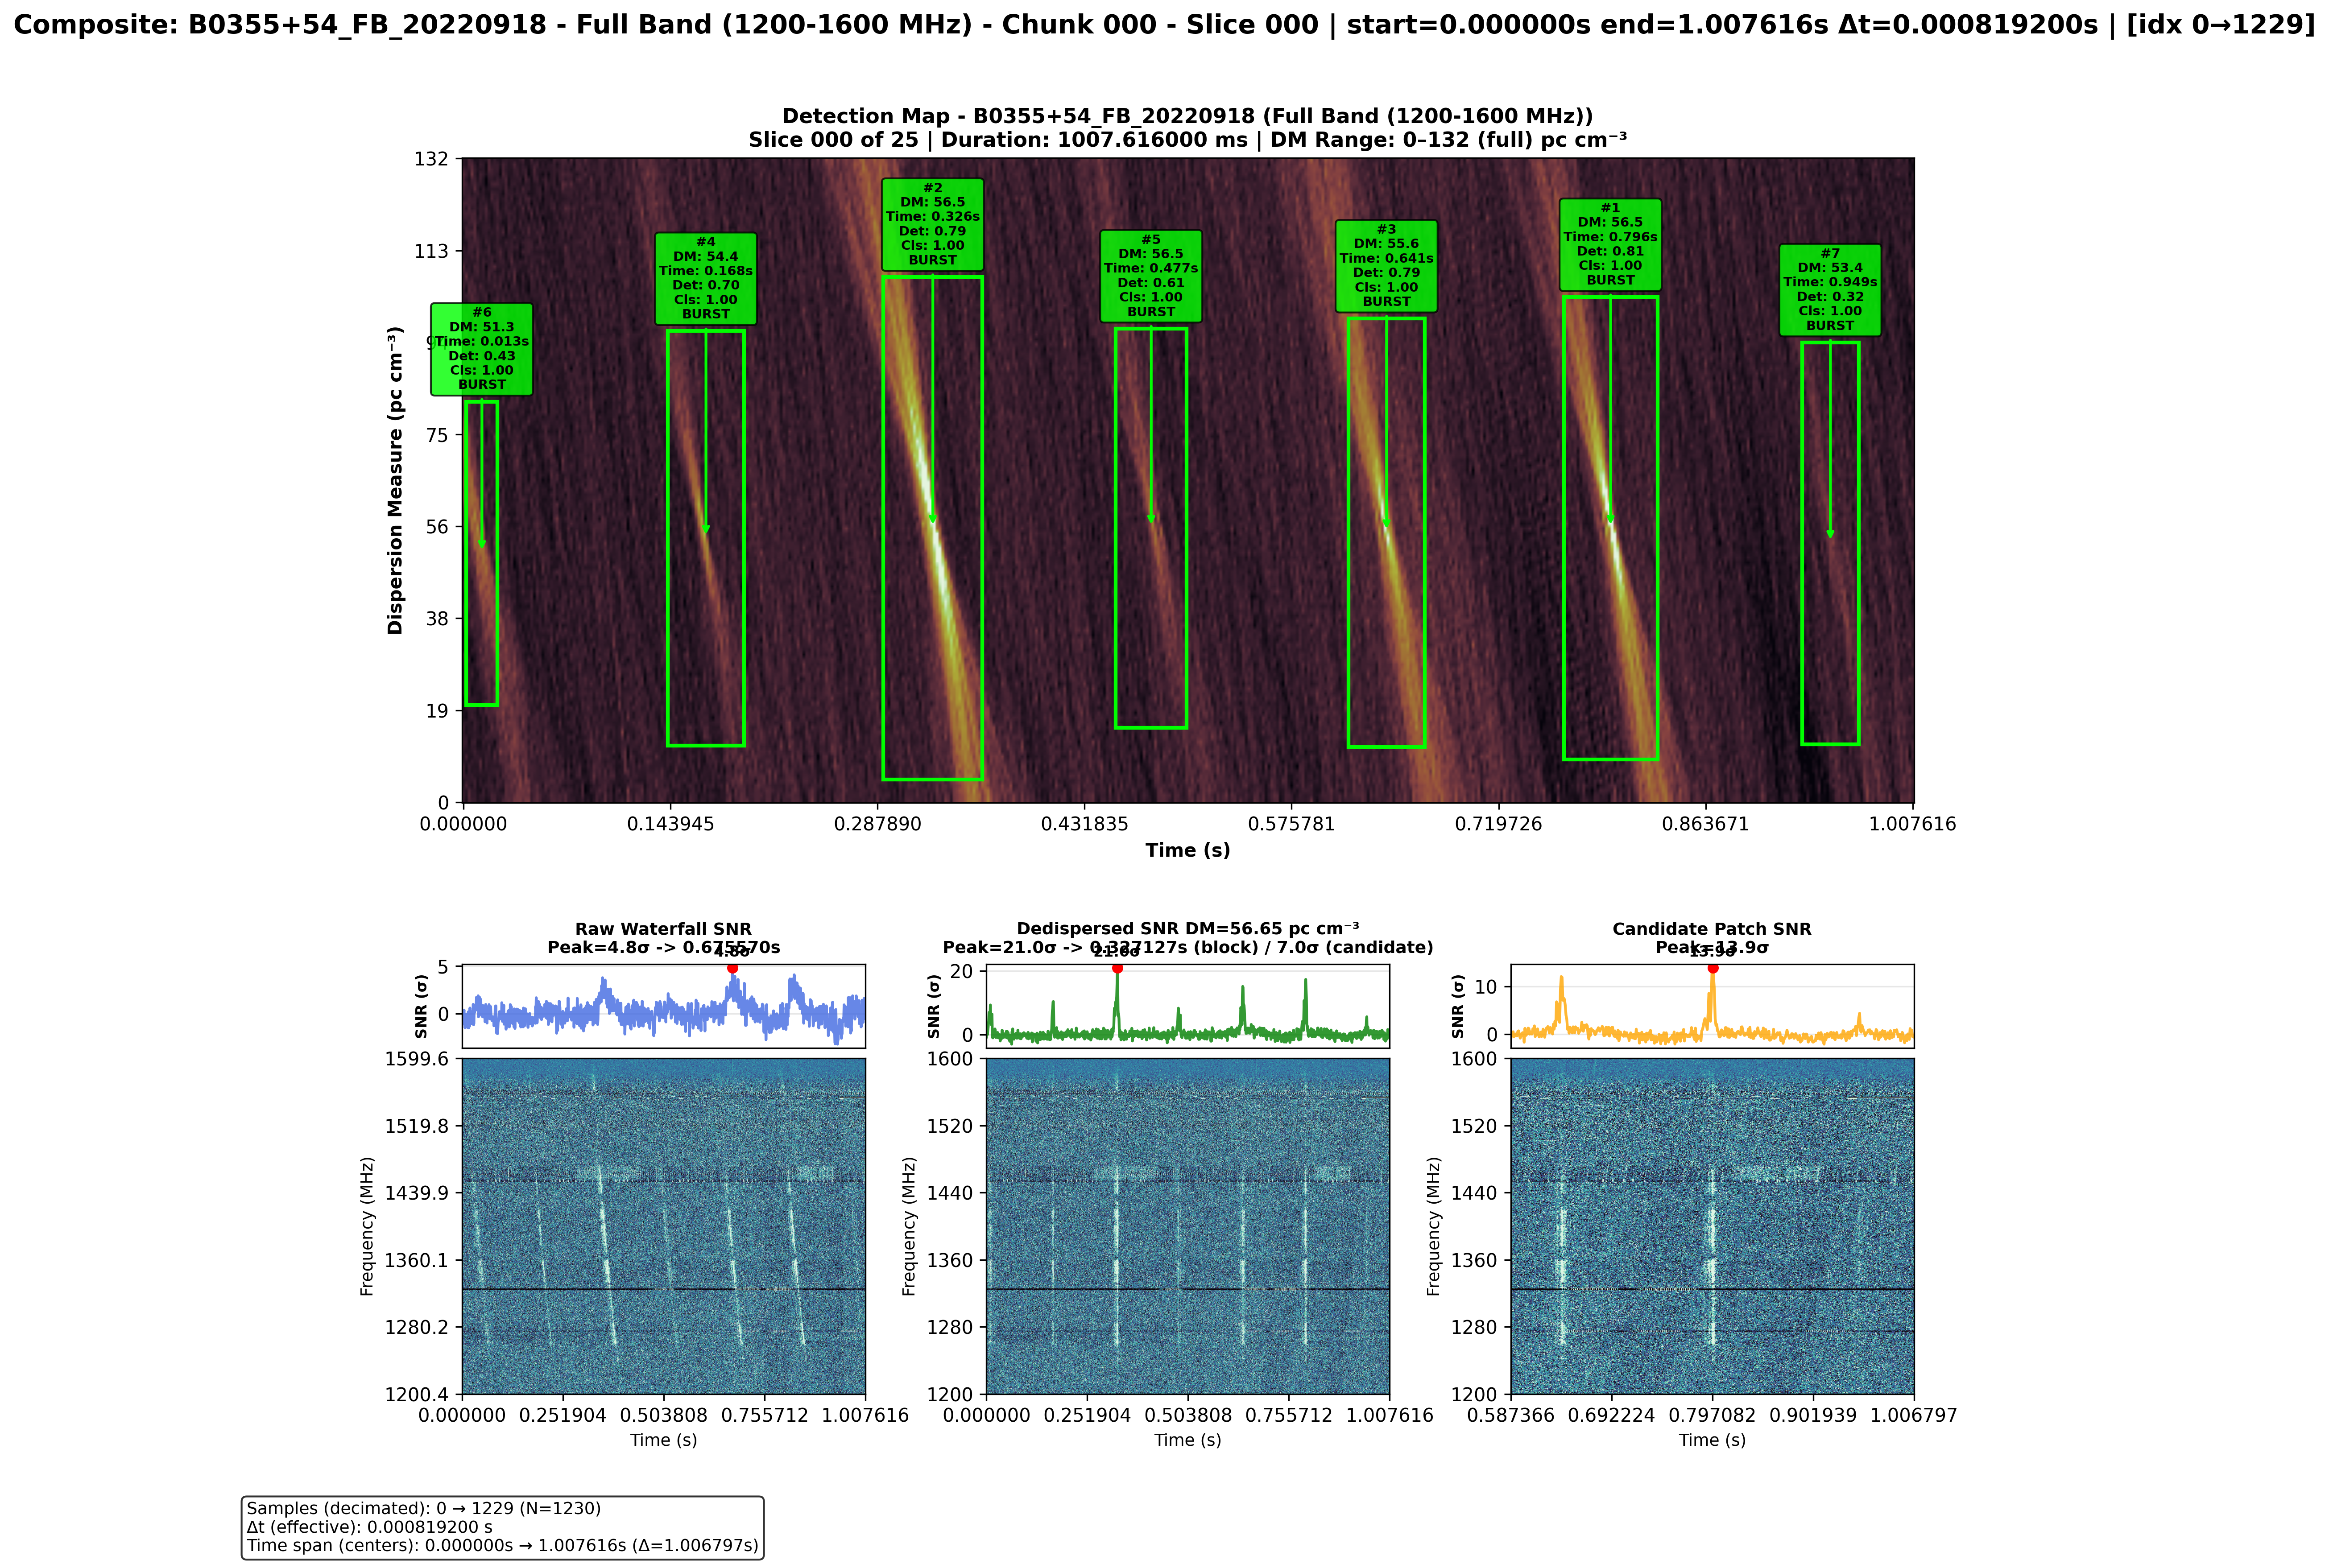
\includegraphics[width=\textwidth]{figures/B0355+54_FB_20220918_slice000.png}
    \caption[Validación continuidad temporal: Slice 000]{7 pulsos detectados en el primer segundo, todos clasificados como BURSTS (scores >0.99).}
    \label{fig:b0355_slice000}
\end{figure}


\begin{figure}[H]
    \centering
    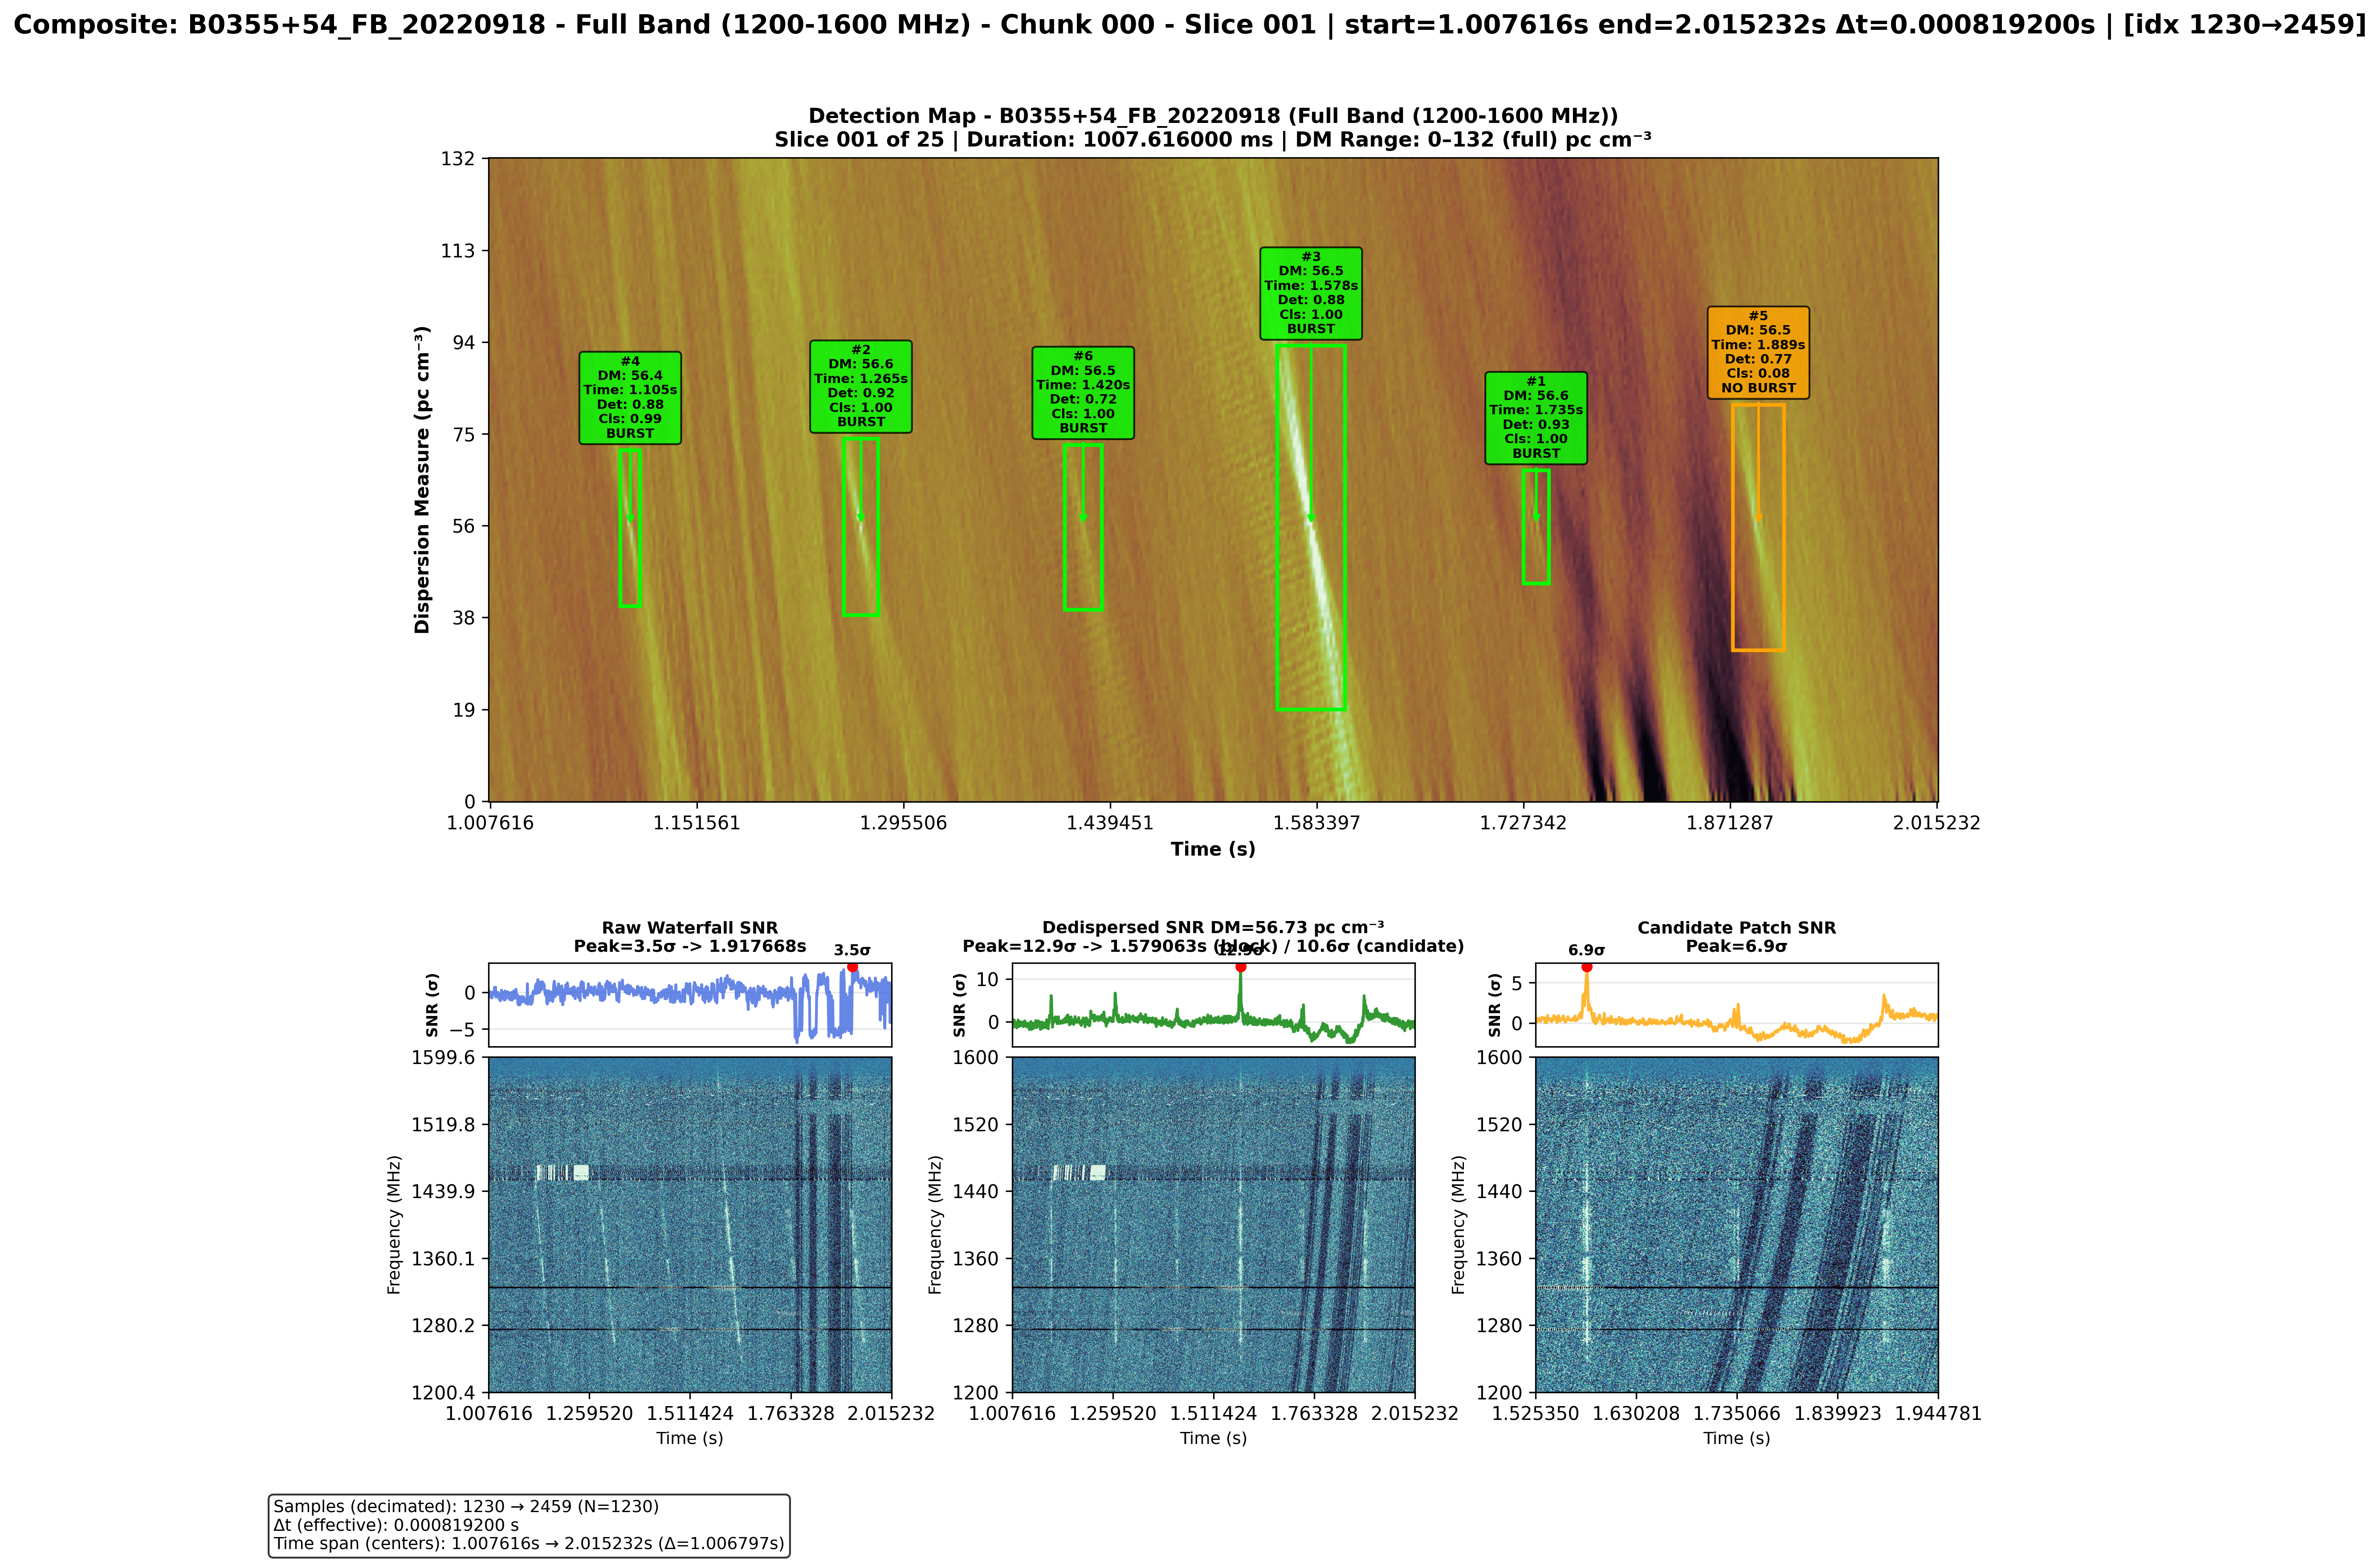
\includegraphics[width=\textwidth]{figures/B0355+54_FB_20220918_slice001.png}
    \caption[Validación continuidad temporal: Slice 001]{5 pulsos clasificados como BURSTS y 1 como NO BURST.}
    \label{fig:b0355_slice001}
\end{figure}

El resultado confirma continuidad temporal y precisión de las redes pre-entrenadas.

\begin{figure}[H]
    \centering
    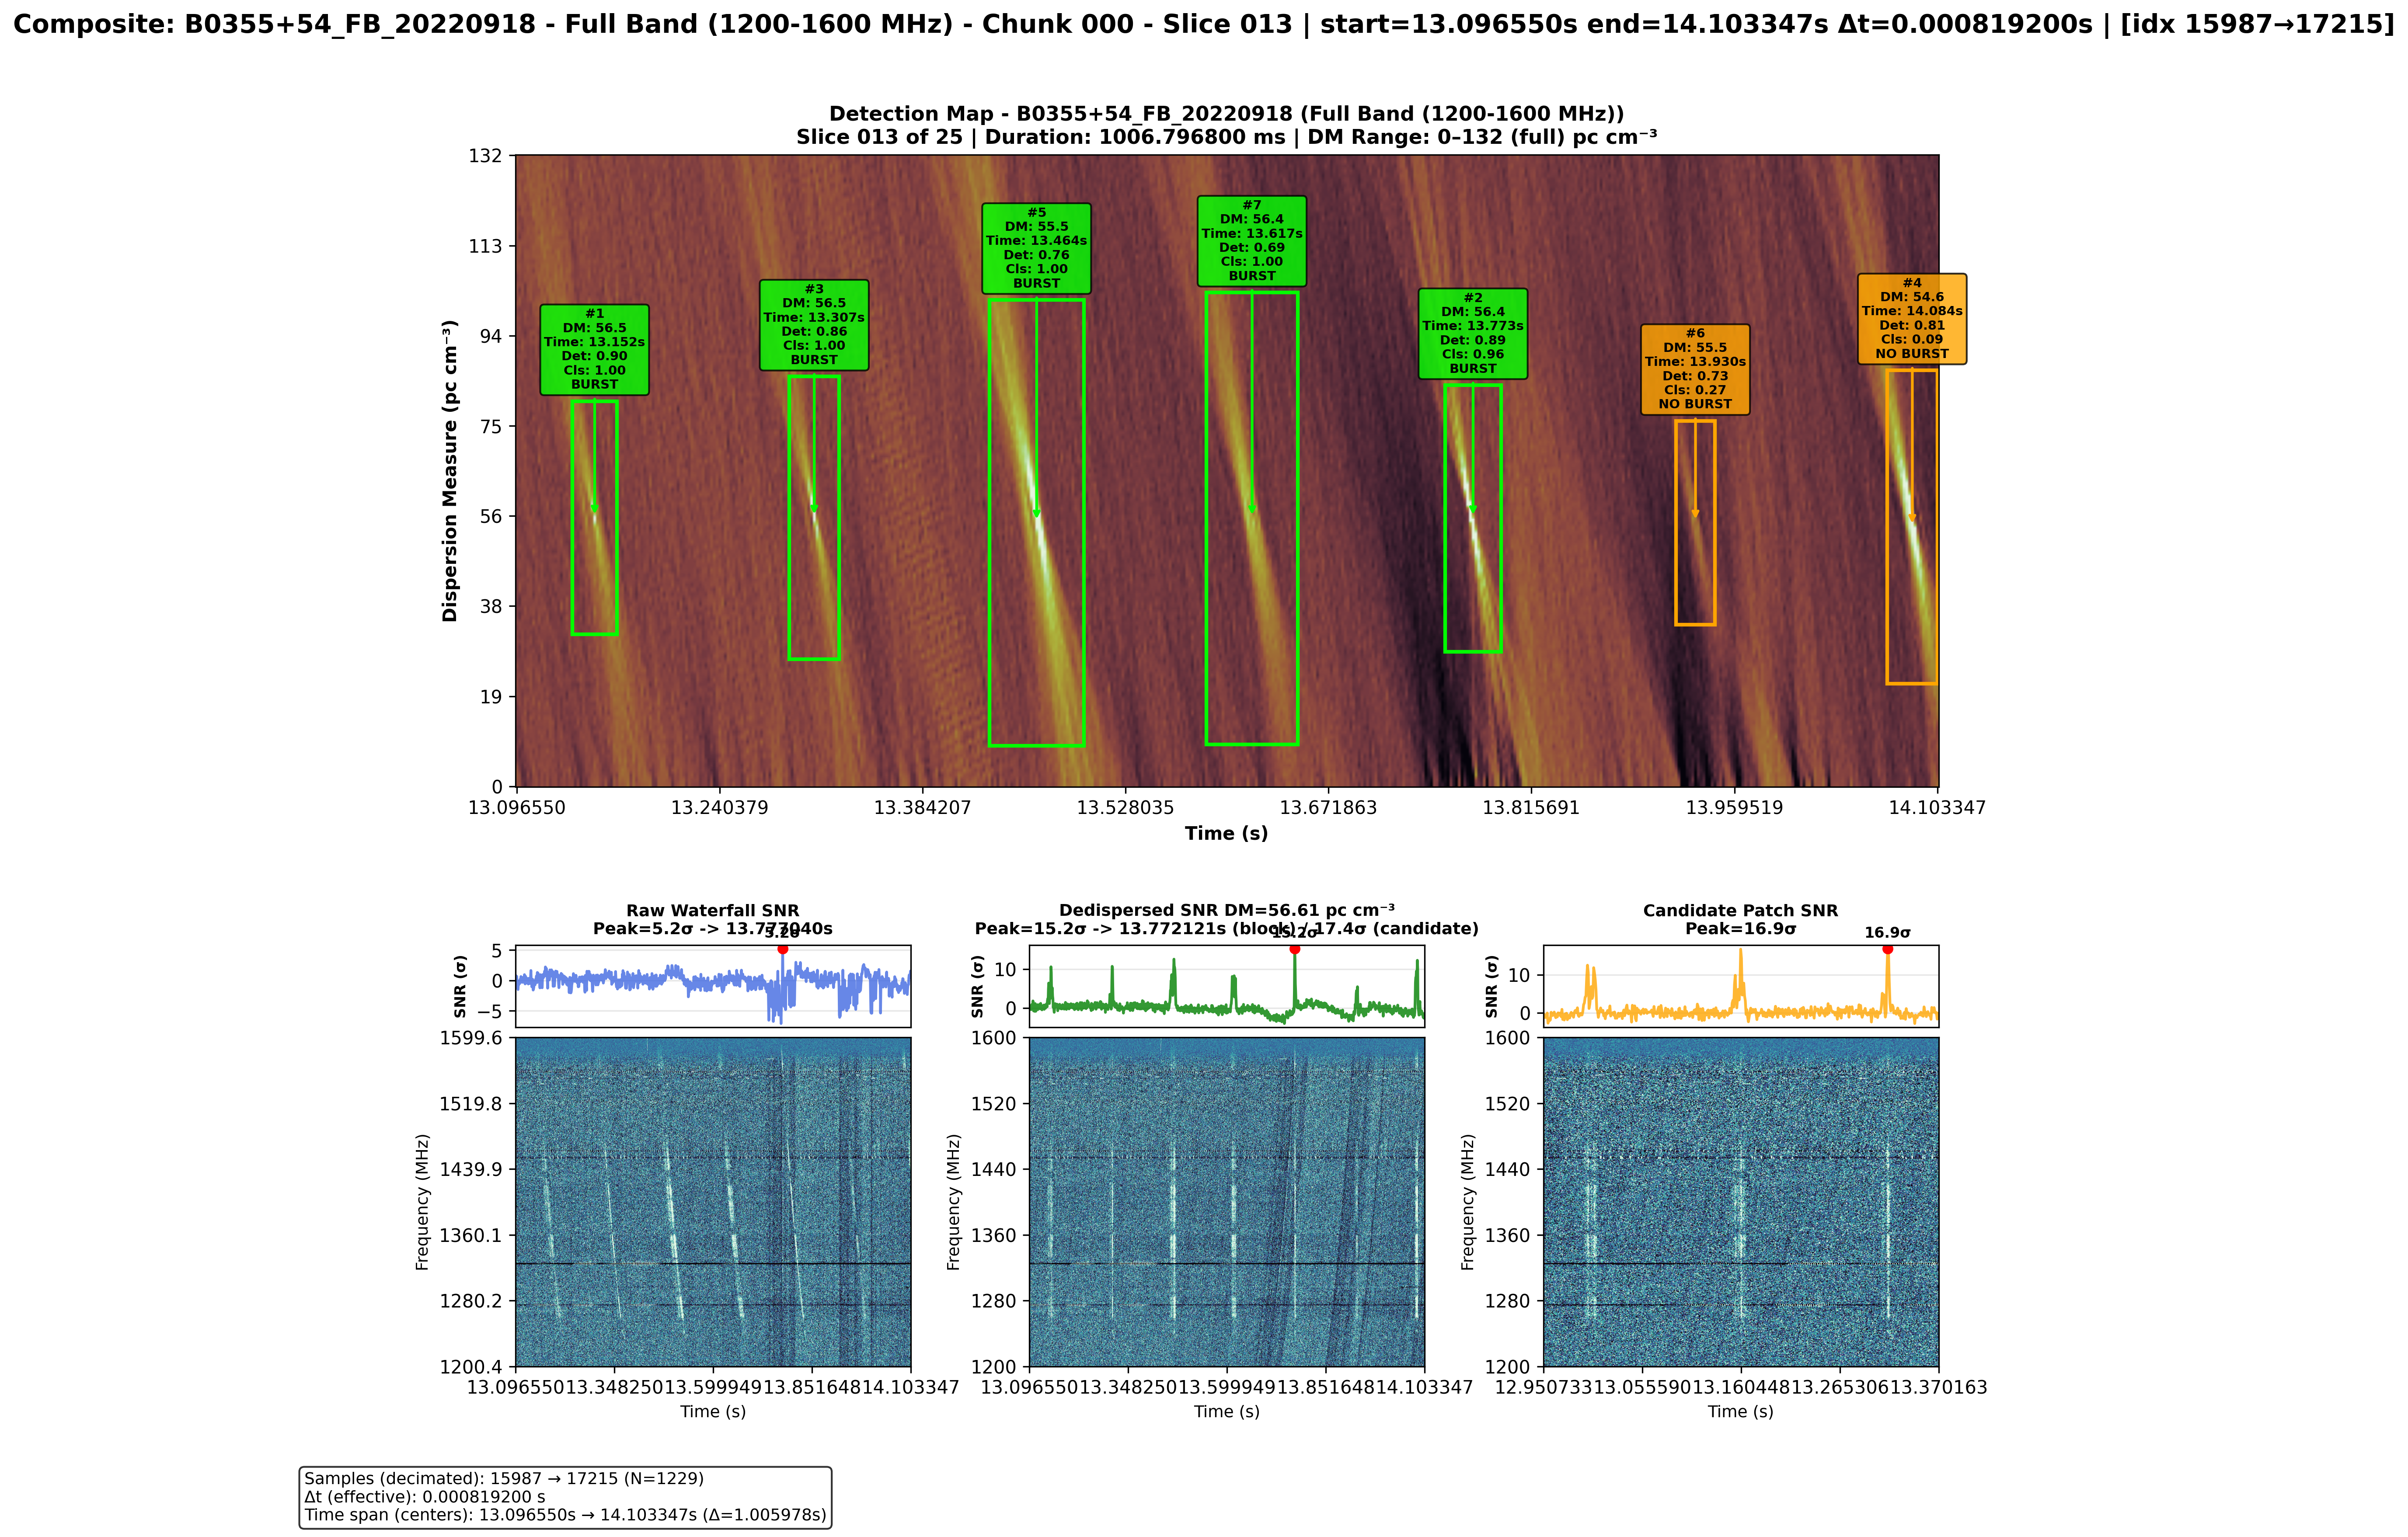
\includegraphics[width=\textwidth]{figures/B0355+54_FB_20220918_slice013.png}
    \caption[Pulso dudoso en la clasificación]{Eventos con alta detección (0.73-0.81) pero baja clasificación (0.09-0.27) clasificados como NO BURST, demostrando capacidad para señales ambiguas.}
    \label{fig:b0355_slice013}
\end{figure}

\subsubsection{Caso 3 - FRB 121102: Validación de Escalabilidad E2E y Descubrimiento Científico}

FRB 121102 valida escalabilidad E2E con archivos multi-gigabyte del radiotelescopio Effelsberg que exceden memoria disponible, forzando operación integrada: ingesta masiva, chunking con solapamiento, gestión inteligente RAM/VRAM y procesamiento E2E sin intervención manual.

Se procesaron 6 archivos observacionales del radiotelescopio Effelsberg de 100m (Alemania) en banda L ($\sim$1.4 GHz), cada uno de $\sim$4 GB en formato PSRFITS, reportados por \cite{cruces2020frb121102}, con ground truth de 24 eventos confirmados. Resultados: 41 eventos detectados, Recall=100\% (24/24 eventos conocidos recuperados), 17 candidatos nuevos identificados, 2 confirmados como genuinos (SNR 6.3$\sigma$ y 12.0$\sigma$, DM$\sim$564 pc cm$^{-3}$).

% Las detecciones completas se documentan en Anexo A: bursts confirmados por literatura (Tabla \ref{tab:anexo_confirmed_bursts}), nuevos eventos confirmados (Tabla \ref{tab:anexo_new_confirmed_bursts}), y candidatos pendientes (Tabla \ref{tab:anexo_candidate_bursts}). El histograma de distribución temporal (Figura \ref{fig:frb121102_histogram}) muestra concentración de eventos en archivos 3098 y 3100, consistente con ventanas de actividad del repetidor.

\begin{figure}[H]
    \centering
    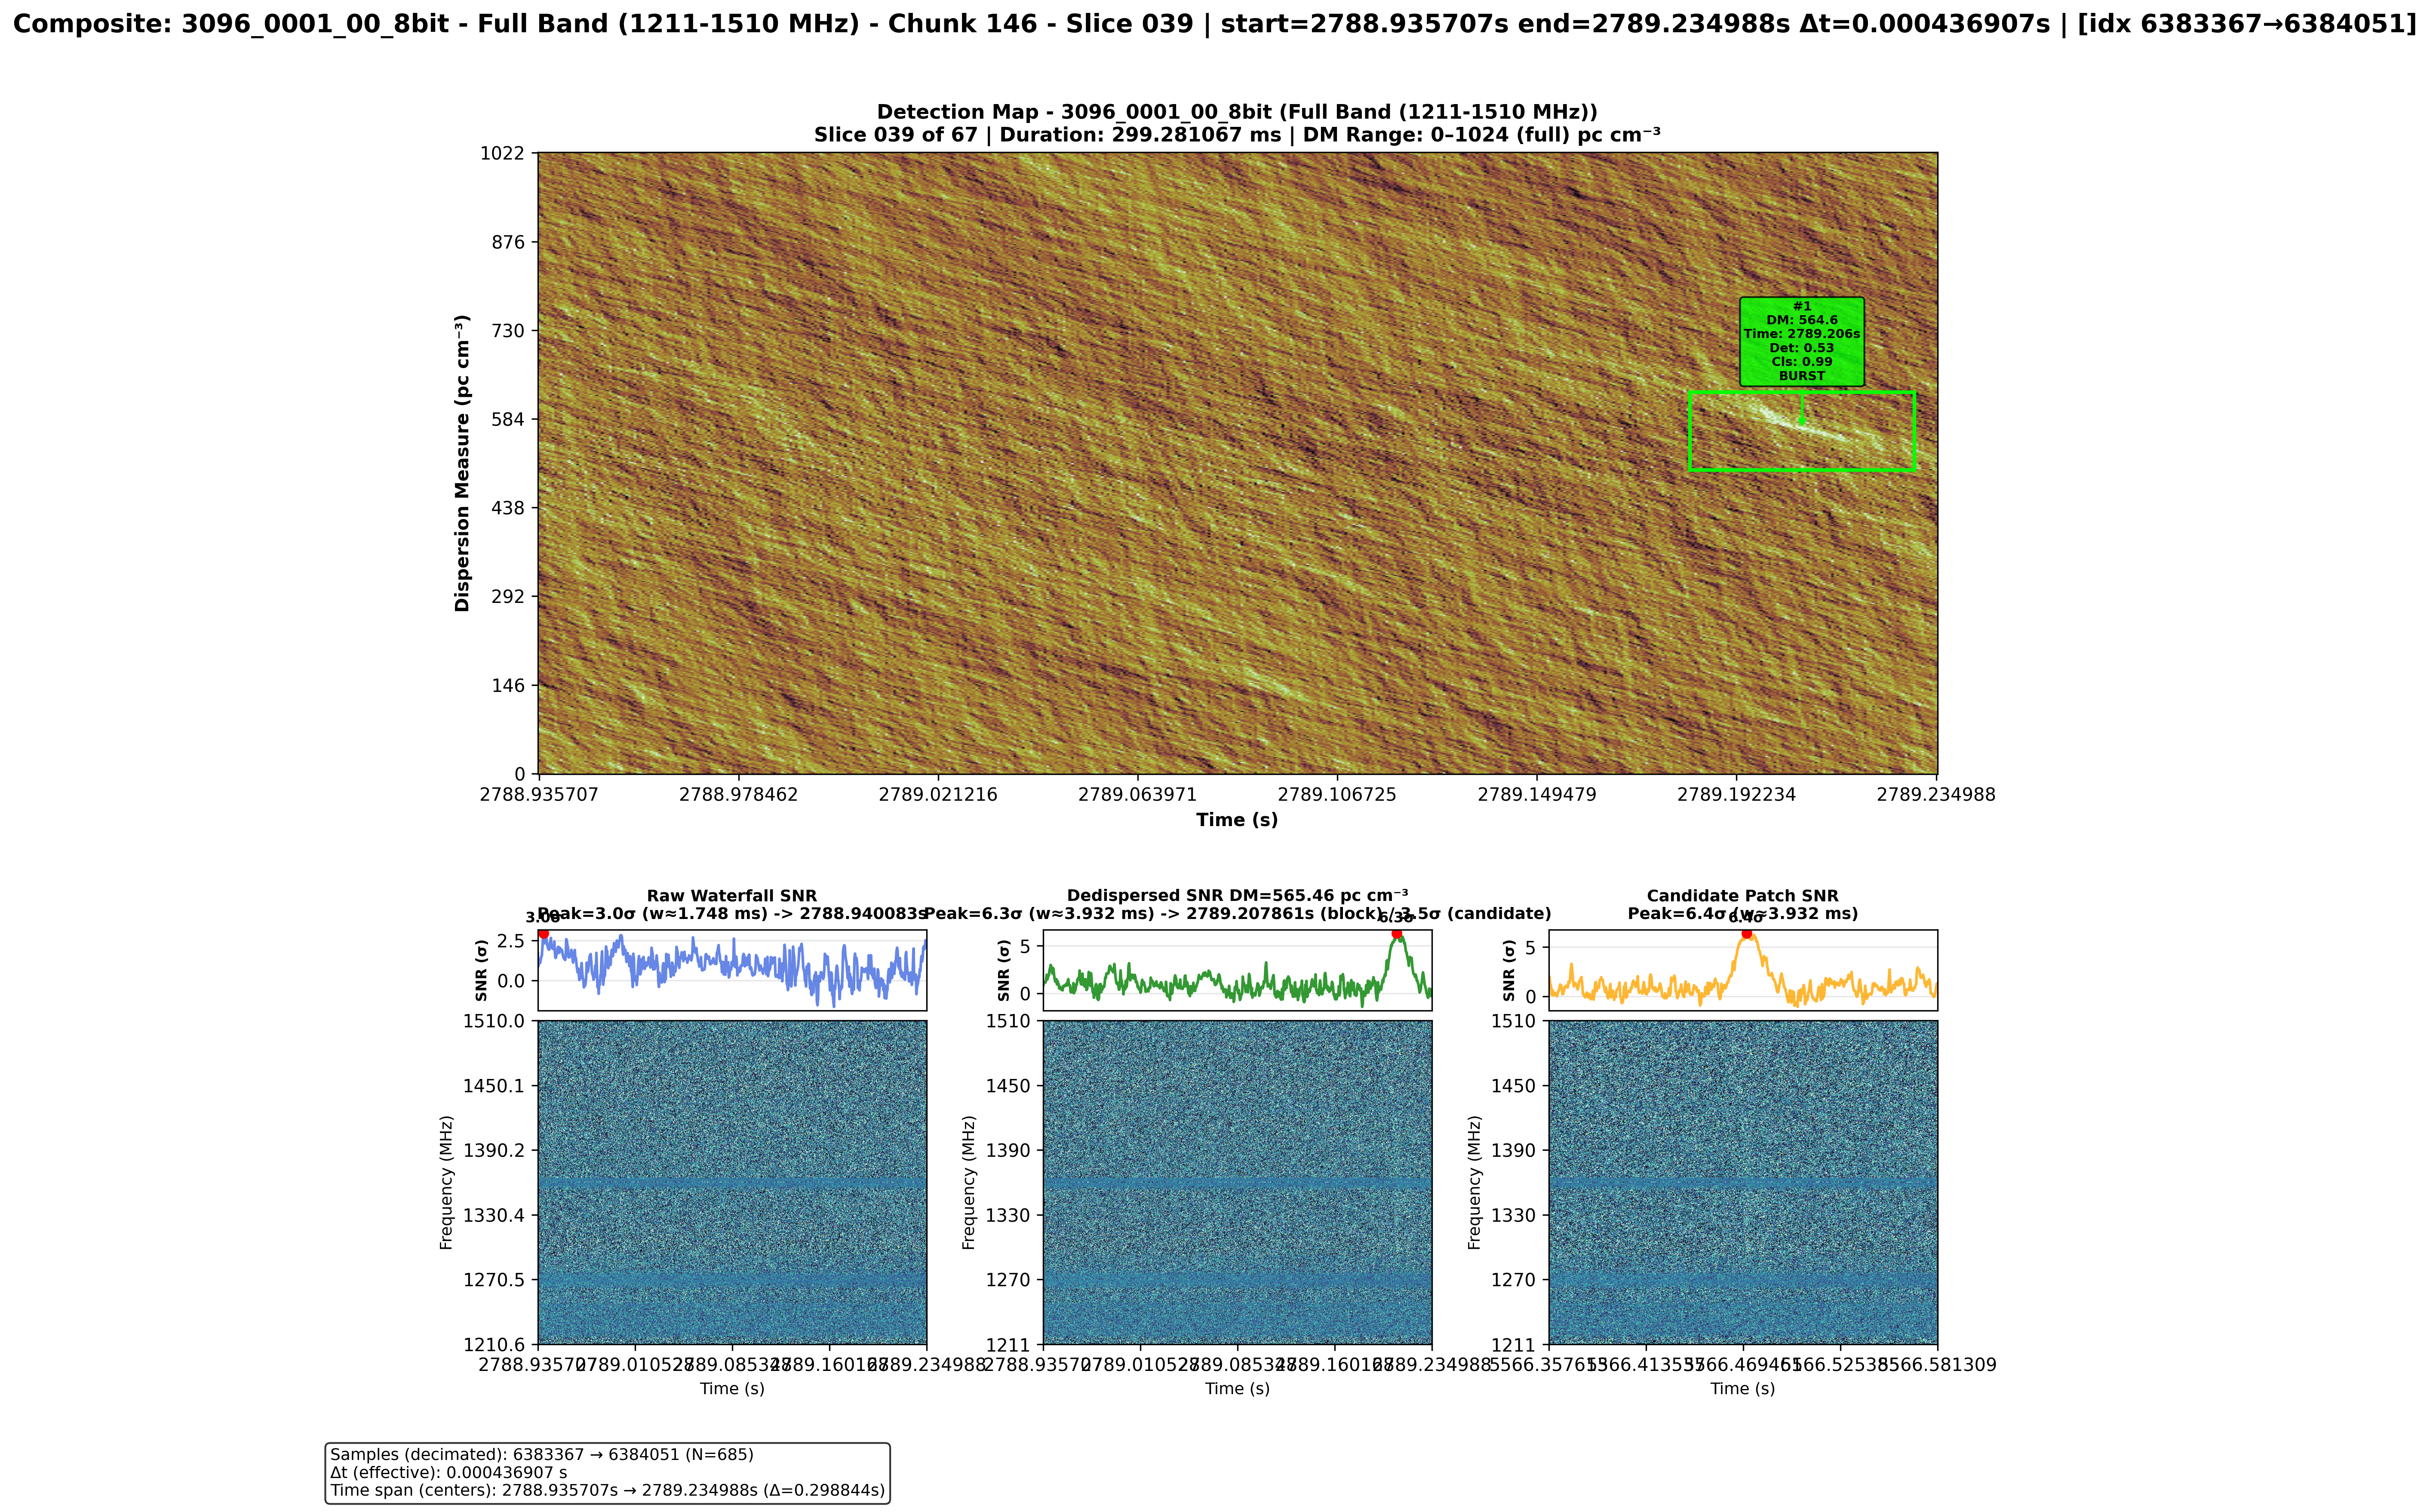
\includegraphics[width=\textwidth]{figures/3096_0001_00_8bit_slice039.png}
    \caption[FRB121102: nuevo evento confirmado (3096\_...\_slice039)]{Primer nuevo evento confirmado: DM=563.6 pc cm$^{-3}$, Time=2421.559296s, SNR=6.3$\sigma$, 100\% confirmado por astrónomos colaboradores.}
    \label{fig:new_event_3096}
\end{figure}

\begin{figure}[H]
    \centering
    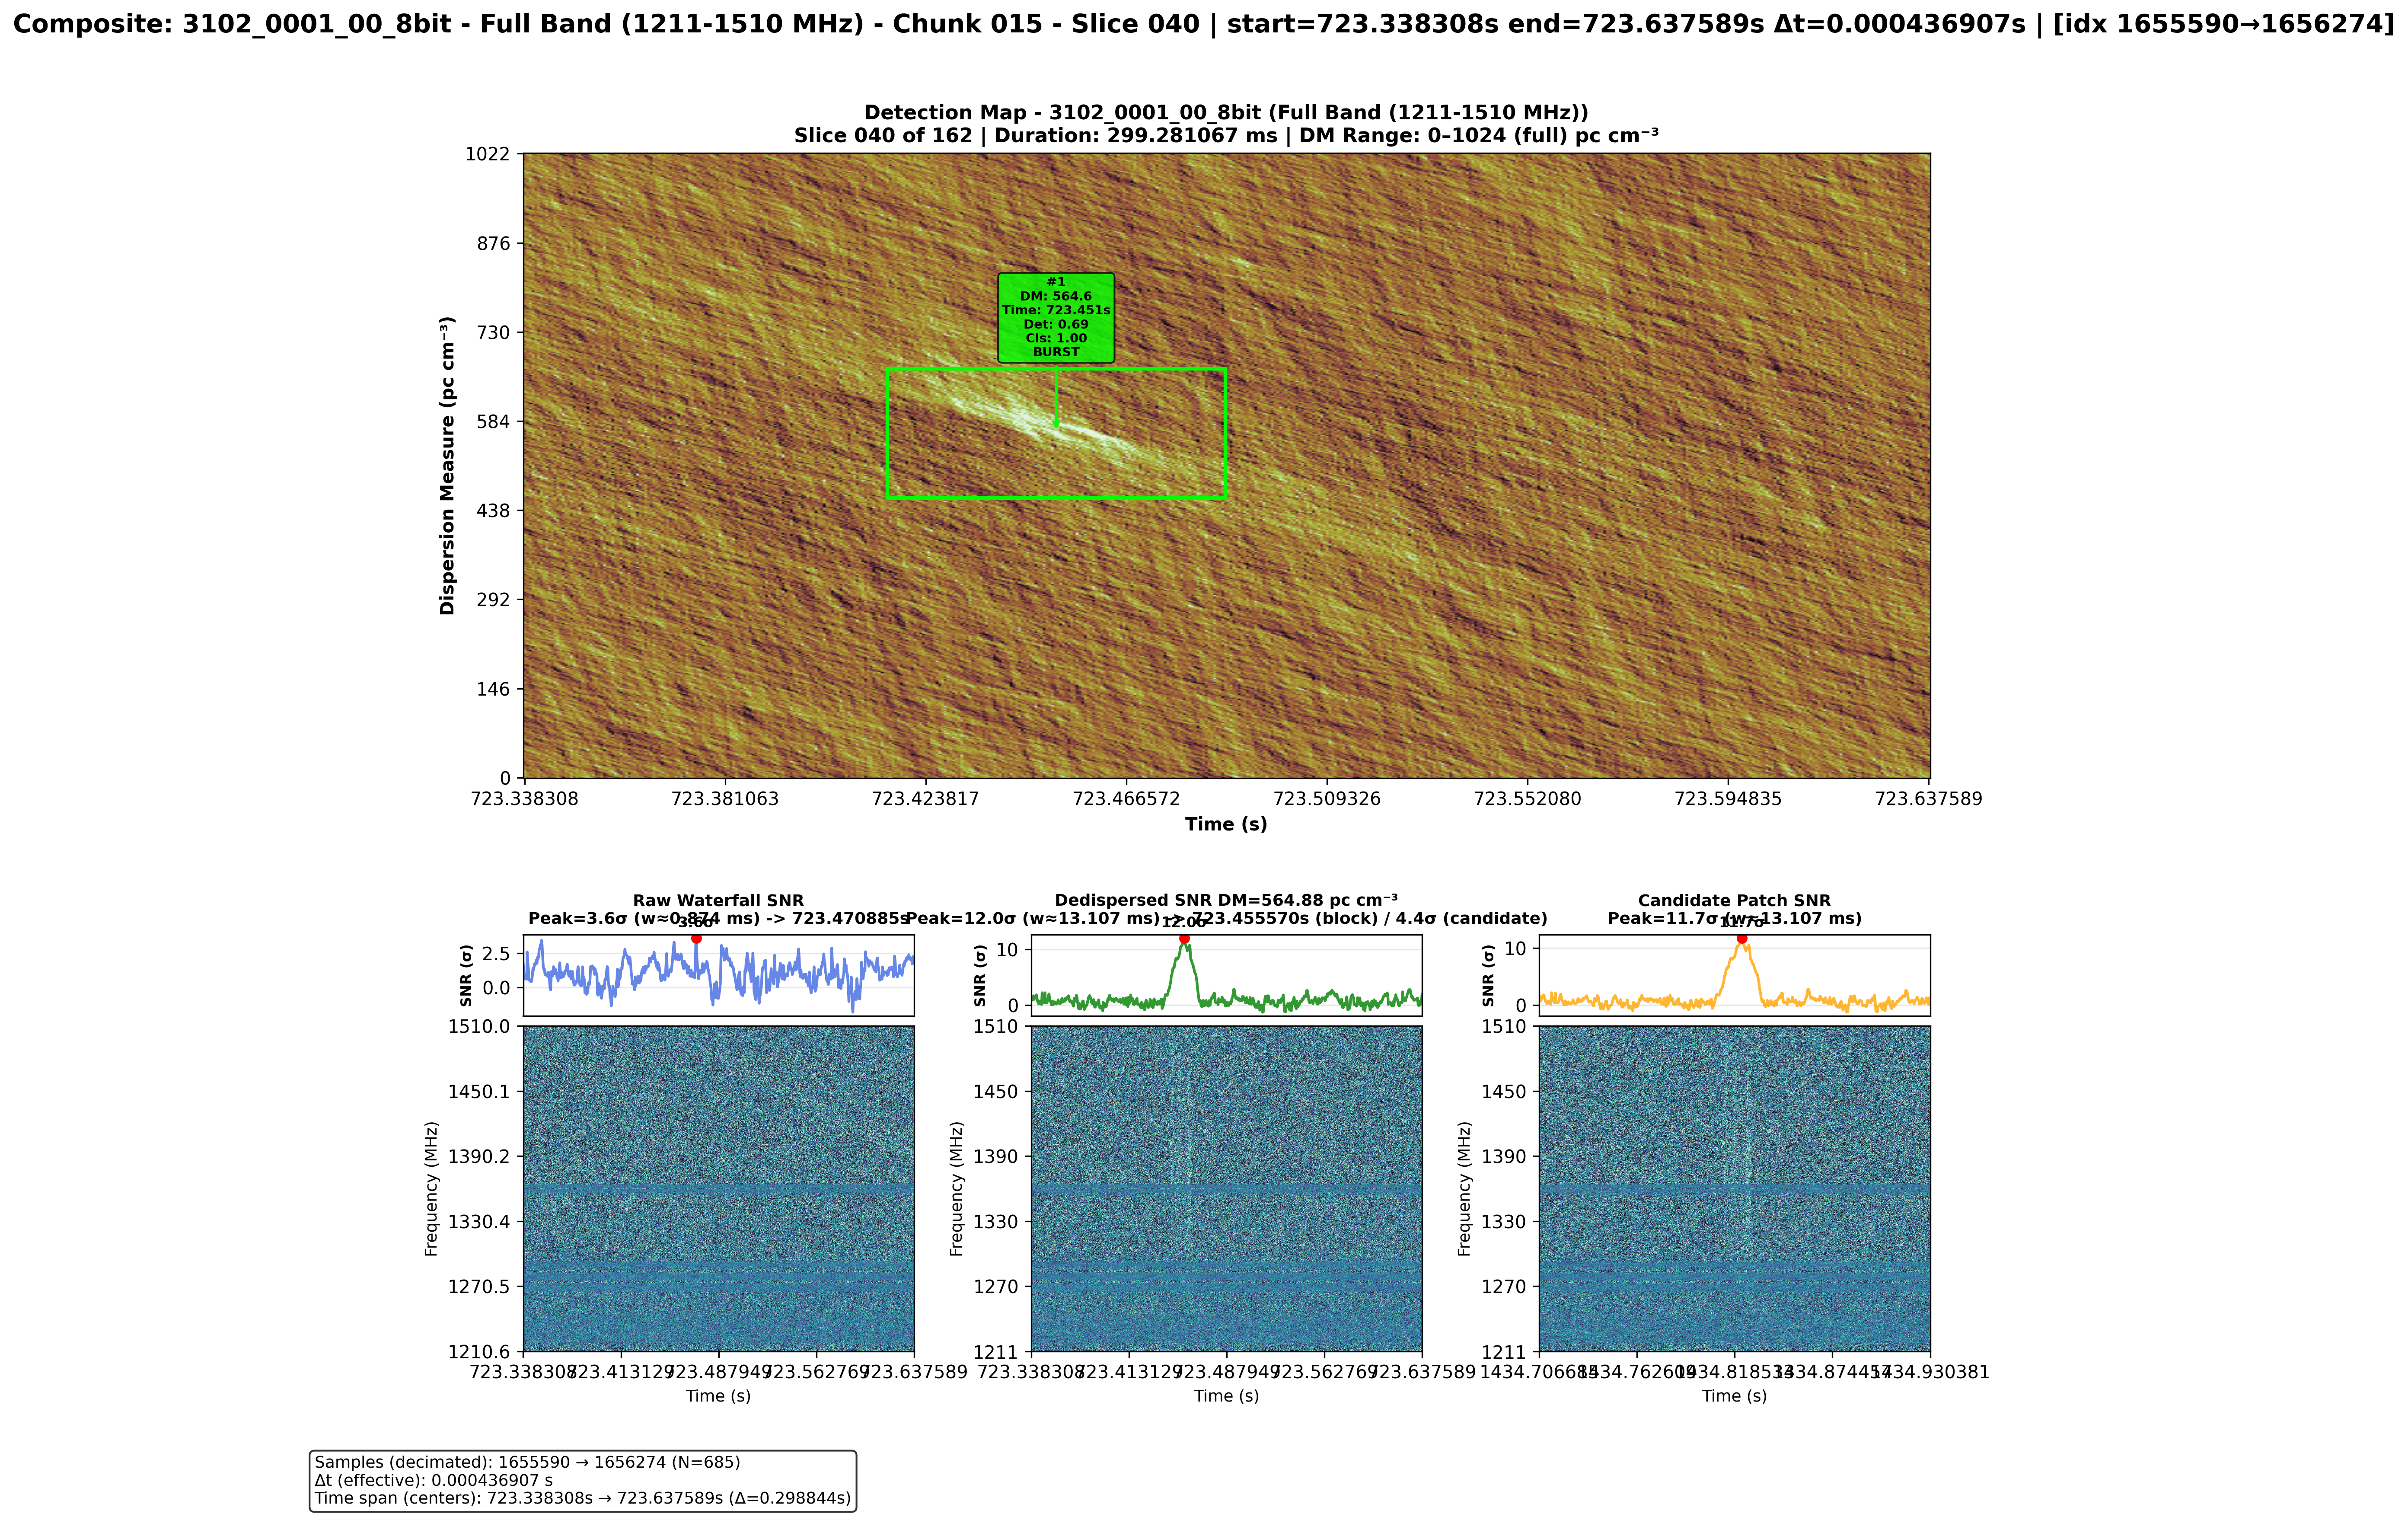
\includegraphics[width=\textwidth]{figures/3102_0001_00_8bit_slice040.png}
    \caption[FRB121102: nuevo evento confirmado (3102\_...\_slice040)]{Segundo nuevo evento confirmado: DM=564.88 pc cm$^{-3}$, Time=723.455399s, SNR=12.0$\sigma$, uno de los bursts más brillantes detectados, 100\% confirmado.}
    \label{fig:new_event_3102}
\end{figure}

% \begin{figure}[H]
%     \centering
%     \includegraphics[width=0.8\textwidth]{figures/frb121102_detection_histogram.png}
%     \caption[Histograma de detecciones FRB121102]{Distribución temporal de detecciones por archivo de observación. Morado: bursts confirmados por literatura; Celeste: nuevos candidatos sin confirmar; Verde: nuevos eventos confirmados. La concentración en archivos 3098 y 3100 es consistente con ventanas de actividad del repetidor. \textit{Fuente: Elaboración propia}.}
%     \label{fig:frb121102_histogram}
% \end{figure}

Los resultados validan integralmente el Componente 1. El pipeline procesó exitosamente archivos multi-gigabyte sin errores de memoria ni degradación de rendimiento, operando sin intervención manual desde ingesta hasta visualización. El recall perfecto (26/26 eventos detectados: 24 de literatura + 2 nuevos confirmados) demuestra que el sistema de chunking con solapamiento controlado no introduce puntos ciegos temporales, validando la continuidad temporal quirúrgica implementada. El descubrimiento de 2 nuevos bursts confirmados demuestra capacidad de descubrimiento científico genuino.

\subsection{VALIDACIÓN DEL COMPONENTE 2: DRAFTS++ - Extensión a Alta Frecuencia - Cuatro Líneas de Investigación}

La validación del Componente 2 examina la efectividad de DRAFTS++ en el régimen milimétrico (86 GHz), donde la firma dispersiva tradicional se comprime significativamente debido a la dependencia $\Delta t_{\mathrm{ms}} \propto \nu^{-2}$. En este régimen, el patrón bow-tie característico de FRBs en bajas frecuencias (1.4 GHz) colapsa, desafiando a detectores entrenados en firmas dispersivas desarrolladas.

Para todas las líneas de investigación se validó utilizando observaciones del Atacama Large Millimeter/submillimeter Array (ALMA, Chile) en modo \emph{phased array}, específicamente datos del magnetar del Centro Galáctico PSR J1745-2900 observados en Banda 3 ($\sim$86 GHz, ancho de banda 2 GHz) durante campañas de 2017, proporcionadas por \cite{veracasanova2025}. Este dataset constituye ground truth mediante 8 pulsos confirmados independientemente con PRESTO (Tabla~\ref{tab:veracasanova_reference}), permitiendo evaluación objetiva de cada estrategia. Los datos fueron adquiridos con resolución temporal de $\sim$8 $\mu$s y formato PSRFITS.

\begin{table}[H]
    \centering
\caption{Ground truth: Pulsos del magnetar PSR J1745-2900 reportados por Vera-Casanova et al. (2025), utilizados para validación de todas las líneas de investigación.}
    \label{tab:veracasanova_reference}
\small
    \begin{tabular}{|c|c|}
        \hline
\textbf{File} & \textbf{Timestamp (s)} \\
        \hline
        142\_0003 & 39.977 \\
142\_0006 & 10.882, 25.829 \\
        153\_0006 & 23.444 \\
230\_0002 & 2.3, 17.395 \\
        230\_0003 & 36.548 \\
        242\_0005 & 44.919 \\
        \hline
\multicolumn{2}{|c|}{Total: 8 pulsos confirmados} \\
\hline
    \end{tabular}
\end{table}

Las métricas de evaluación son estándar: Recall, que mide sensibilidad (fracción de pulsos genuinos detectados), Precision, que cuantifica especificidad (proporción de detecciones correctas), y F1-score que sintetiza el balance entre ambas. Los resultados se complementan con análisis de casos representativos que ilustran modos de éxito y falla de cada estrategia.

\subsubsection{Línea 1: Validación de Transferibilidad del Pipeline Clásico mediante Adaptación Paramétrica}

Esta línea establece el baseline de rendimiento del pipeline clásico (CenterNet + ResNet18) en alta frecuencia sin modificaciones arquitecturales, evaluando si ajustes paramétricos simples pueden compensar la compresión del bow-tie. El experimento compara dos configuraciones de umbral de detección: conservadora (DET\_PROB = 0.3, optimizada en bajas frecuencias) y sensible (DET\_PROB = 0.05, factor x6 más permisivo), aislando el efecto del umbral sobre sensibilidad y especificidad.

Los resultados revelaron comportamiento bimodal dramático. Con el umbral estándar (DET\_PROB = 0.3), el sistema falló completamente: ninguno de los 8 pulsos de referencia fue detectado. Este resultado confirma que modelos optimizados para bow-ties desarrollados no transfieren directamente a regímenes comprimidos, independientemente de la calidad del entrenamiento original.

Al reducir el umbral en factor x6 (DET\_PROB = 0.05), el sistema recuperó sensibilidad parcial detectando 7/8 pulsos (Recall = 87.5\%), pero introdujo aproximadamente 12 candidatos espurios, degradando la precisión a 36.8\%. El F1-score de 51.8\% refleja el trade-off fundamental entre sensibilidad y especificidad inherente a la adaptación paramétrica: ajustar el umbral desplaza el punto de operación en la curva ROC pero no expande el dominio de representación del modelo. La Tabla \ref{tab:comparacion_umbrales_linea1} sintetiza estas métricas.

\begin{table}[H]
    \centering
    \caption{Rendimiento del pipeline clásico adaptado según configuración de umbral. Las métricas cuantifican el trade-off fundamental entre sensibilidad (recall) y especificidad (precision) en adaptación paramétrica para alta frecuencia. \textit{Fuente: Elaboración propia}.}
    \label{tab:comparacion_umbrales_linea1}
    \begin{tabular}{|l|c|c|}
        \hline
        \textbf{Métrica} & \textbf{Conservadora} & \textbf{Sensible} \\
         & \textbf{(DET\_PROB = 0.3)} & \textbf{(DET\_PROB = 0.05)} \\
        \hline
        Recall & 0\% (0/8) & 87.5\% (7/8) \\
        \hline
        Precision & Indefinida & 36.8\% (7/19) \\
        \hline
        F1-Score & Indefinida & 51.8\% \\
        \hline
        Falsos Positivos & 0 & ~12 (estimado) \\
        \hline
        Caracterización & Específico/Insensible & Sensible/Impreciso \\
        \hline
    \end{tabular}
\end{table}

Dos casos ilustran el espectro de comportamientos observados. El primer pulso (Archivo 142\_0003, t=39.977s) no fue detectado con umbral conservador (Figura \ref{fig:142_0003_slice133_highProb}), pero apareció con probabilidad marginal 9\% al reducir el umbral (Figura \ref{fig:142_0003_slice133_lowProb}). Este éxito parcial sugiere que el modelo captura características relevantes de alta frecuencia, aunque requiere umbral permisivo para activarse. El costo es evidente: candidatos espurios adicionales emergen simultáneamente, introduciendo ruido de clasificación.

El segundo caso (Archivo 242\_0005, t=44.169s) permaneció indetectable en ambas configuraciones (Figuras \ref{fig:242_0005_slice149_highProb} y \ref{fig:242_0005_slice149_lowProb}). Esta falla persistente revela limitaciones arquitecturales irreductibles: ciertas señales de alta frecuencia escapan completamente al dominio de representación aprendido por el modelo, independientemente de ajustes paramétricos.

\begin{figure}[H]
    \centering
    \includegraphics[width=0.9\textwidth]{figures/2017-04-03-08-16-13_142_0003_t39.977_slice133.png}
    \caption[Caso A: Configuración conservadora]{Caso A con configuración conservadora (DET\_PROB = 0.3). El mapa de detección DM-tiempo muestra ausencia total de candidatos para el pulso confirmado en t=39.977s. El umbral estándar optimizado para bajas frecuencias resulta incompatible con características espectrales de alta frecuencia. \textit{Fuente: Elaboración propia}.}
    \label{fig:142_0003_slice133_highProb}
\end{figure}

\begin{figure}[H]
    \centering
    \includegraphics[width=0.9\textwidth]{figures/2017-04-03-08-16-13_142_0003_t39.977_slice133-lowProb.png}
    \caption[Caso A: Configuración sensible]{Caso A con configuración sensible (DET\_PROB = 0.05). El sistema detecta el pulso genuino en t=39.976s con probabilidad marginal 9\%, junto con candidatos espurios adicionales. La recuperación de detección mediante reducción de umbral demuestra sensibilidad paramétrica, pero a costa de especificidad reducida. \textit{Fuente: Elaboración propia}.}
    \label{fig:142_0003_slice133_lowProb}
\end{figure}

\begin{figure}[H]
    \centering
    \includegraphics[width=0.9\textwidth]{figures/2017-04-03-13_38_31_242_0005_t44.169_slice149.png}
    \caption[Caso B: Configuración conservadora]{Caso B con configuración conservadora (DET\_PROB = 0.3). Ausencia total de detecciones para pulso confirmado en t=44.169s, consistente con falla sistemática observada en configuración estándar. \textit{Fuente: Elaboración propia}.}
    \label{fig:242_0005_slice149_highProb}
\end{figure}

\begin{figure}[H]
    \centering
    \includegraphics[width=0.9\textwidth]{figures/2017-04-03-13_38_31_242_0005_t44.169_slice149-lowProb.png}
    \caption[Caso B: Configuración sensible]{Caso B con configuración sensible (DET\_PROB = 0.05). A pesar del umbral extremadamente permisivo, el pulso confirmado permanece indetectable. Esta falla persistente evidencia limitaciones arquitecturales fundamentales: ciertas características espectrales de alta frecuencia escapan al dominio de aplicación del modelo pre-entrenado, independientemente de ajustes paramétricos. \textit{Fuente: Elaboración propia}.}
    \label{fig:242_0005_slice149_lowProb}
\end{figure}
Los resultados establecen el límite superior del pipeline clásico en alta frecuencia: Recall máximo 87.5\% con Precision 36.8\%. El umbral estándar (0\% recall) resulta completamente inadecuado, mientras que el umbral permisivo recupera sensibilidad a costa de especificidad degradada. 


\subsubsection{Línea 2: Validación de Estrategia Híbrida SNR-Threshold + Clasificación CNN}

Enfoque híbrido inspirado en PRESTO: propuesta por SNR-threshold seguida de clasificación ResNet18. Pipeline: (i) detección picos SNR con filtrado adaptado (boxcar $w \in \{1,\ldots,30\}$, umbral 6-10$\sigma$), (ii) estimación $\mathrm{DM}^*$ por coherencia temporal, (iii) clasificación binaria del patch dedispersado. Validación cruzada incluye 8 pulsos PRESTO adicionales.

Resultados: Recall=100\% (8/8 pulsos literatura + 8/8 PRESTO), superando Línea 1 (87.5\% máx). El sistema descubrió 44 nuevos pulsos confirmados (×5.5 censo conocido) y 101 candidatos prometedores pendientes validación polarimétrica (161 eventos totales). Métricas globales: Recall=100\%, Precision=37.3\%, F1=54.4\%, manteniendo precisión similar a Línea 1 (36.8\%) pero con recall perfecto (Tabla \ref{tab:comparacion_lineas_alma}).

\begin{table}[H]
    \centering
    \caption{Comparación cuantitativa Línea 1 vs. Línea 2. El enfoque híbrido (Línea 2) supera dramáticamente al pipeline clásico adaptado (Línea 1), logrando recall perfecto (100\%) y descubriendo 44 eventos nuevos confirmados. \textit{Fuente: Elaboración propia}.}
    \label{tab:comparacion_lineas_alma}
    \begin{tabular}{|l|c|c|}
        \hline
        \textbf{Métrica} & \textbf{Línea 1 (DM-Tiempo)} & \textbf{Línea 2 (SNR-Híbrido)} \\
        \hline
        Recall (Literatura) & 87.5\% (7/8) & 100\% (8/8) \\
        \hline
        Recall (PRESTO) & 0\% (0/8) & 100\% (8/8) \\
        \hline
        Precision & 36.8\% & 37.3\% \\
        \hline
        F1-Score & 51.8\% & 54.4\% \\
        \hline
        Nuevos Confirmados & 0 & 44 \\
        \hline
        Candidatos Prometedores & ~12 & 101 \\
        \hline
    \end{tabular}
\end{table}

Las Figuras \ref{fig:alma_presence_validation_1}--\ref{fig:alma_new_candidate_validation} ilustran detecciones representativas, incluyendo re-detecciones de pulsos PRESTO y nuevos descubrimientos con morfología excepcional.

\begin{figure}[H]
    \centering
    \includegraphics[width=0.95\textwidth]{figures/DRAFTS-HF-SNR/2017-04-03-12_56_05_230_0003_t36.548_slice121.png}
    \caption[Re-detección PRESTO: Archivo 230\_0003]{Re-detección exitosa de pulso PRESTO (Archivo 230\_0003, t=36.548s). El enfoque híbrido detectó dos componentes con DM=46.9 pc cm$^{-3}$ y clasificación "BURST" (scores 1.00). Los paneles inferiores muestran transformación de señal dispersa (Raw Waterfall) a dedispersada (Dedispersed SNR), con picos 13.8$\sigma$ y 15.8$\sigma$. \textit{Fuente: Elaboración propia}.}
    \label{fig:alma_presence_validation_1}
\end{figure}

\begin{figure}[H]
    \centering
    \includegraphics[width=0.95\textwidth]{figures/DRAFTS-HF-SNR/2017-04-03-08_16_13_0003_slice133.png}
    \caption[Re-detección PRESTO: Archivo 142\_0003]{Re-detección exitosa de pulso PRESTO (Archivo 142\_0003, t=39.977s). El enfoque híbrido detectó tres componentes con DM=46.9 pc cm$^{-3}$ y clasificación "BURST" (scores 1.00). SNR dedispersado muestra pico 9.0$\sigma$ (block) / 8.2$\sigma$ (candidate). Este pulso fue indetectable en Línea 1 con configuración conservadora. \textit{Fuente: Elaboración propia}.}
    \label{fig:alma_presence_validation_2}
\end{figure}

\begin{figure}[H]
    \centering
    \includegraphics[width=0.95\textwidth]{figures/DRAFTS-HF-SNR/2017-04-03-08_16_13_0001_slice143.png}
    \caption[Nuevo descubrimiento: Archivo 142\_0001]{Ejemplo de nuevo candidato prometedor (Archivo 142\_0001, t=43.136s). El candidato muestra DM=46.9 pc cm$^{-3}$, clasificación "BURST" (score 1.00), y picos SNR excepcionales de 9.4$\sigma$ (raw/dedispersado) y 10.3$\sigma$ (candidate). Morfología claramente distinguible en waterfalls. Representa uno de 101 candidatos prometedores pendientes de validación polarimétrica completa. \textit{Fuente: Elaboración propia}.}
    \label{fig:alma_new_candidate_validation}
\end{figure}

Los resultados validan la estrategia híbrida: el clasificador ResNet18 transfiere exitosamente a alta frecuencia (scores ~1.00 para pulsos genuinos), mientras que la propuesta SNR-threshold recupera completamente todos los pulsos conocidos (16/16), superando el límite de Línea 1 (87.5\%). El descubrimiento de 44 nuevos pulsos confirmados ( x5.5 respecto a literatura) demuestra capacidad de descubrimiento científico genuino. La Precision moderada (37.3\%) refleja filosofía de diseño apropiada para sistemas exploratorios: sensibilidad máxima tolerando candidatos prometedores pendientes de validación polarimétrica.

\paragraph{Caso Excepcional: Detección de Pulso Único con Morfología Temporal Extendida}

La Línea 2 detectó un pulso único del magnetar PSR J1745-2900 con morfología temporal extendida manifestado como 13 componentes temporales en ~0.6s (slices consecutivos del archivo 2017-04-03-12\_47\_05\_0002, ventana 2s, downsampling 1080). Todos los componentes muestran DM=46.9 pc cm$^{-3}$ y clasificación BURST (scores 1.00). El slice 036 presenta 7 componentes (SNR 6.1-7.3$\sigma$), mientras el slice 037 muestra 6 componentes adicionales (SNR 8.3$\sigma$, ancho ~30.7 ms).

Esta estructura temporal compleja sugiere dispersión intrínseca por plasma circumpulsar, scattering múltiple interestelar, o emisión con haz complejo. El análisis polarimétrico (Figura \ref{fig:pulso_polarimetrico}) confirma polarización lineal dominante (~13-14$\sigma$) sobre circular (~4-5$\sigma$) con espectro de banda ancha uniforme (85.25-87.00 GHz).

El enfoque híbrido demuestra capacidad para resolver estructura temporal fina, mantener especificidad alta identificando múltiples componentes del mismo evento, y capturar pulsos de ancho atípico que escapan a detectores basados solo en patrones dispersivos.

\begin{figure}[H]
    \centering
    \includegraphics[width=0.9\textwidth]{figures/DRAFTS-HF-SNR/2017-04-03-12_47_05_0002_slice036.png}
    \caption[Componentes temporales - Slice 036]{7 componentes temporales en slice 036 (10.801-11.101s): DM=46.9 pc cm$^{-3}$, clasificación 1.00, SNR 6.1-7.3$\sigma$. Estructura extendida sugiere dispersión circumpulsar.}
    \label{fig:slice036_multiple_detections}
\end{figure}

\begin{figure}[H]
    \centering
    \includegraphics[width=0.9\textwidth]{figures/DRAFTS-HF-SNR/2017-04-03-12_47_05_0002_slice037.png}
    \caption[Componentes temporales - Slice 037]{6 componentes adicionales en slice 037 (11.101-11.401s): DM=46.9 pc cm$^{-3}$, clasificación perfecta, SNR 8.3$\sigma$, ancho ~30.7 ms. Secuencia completa (13 componentes, ~0.6s) evidencia resolución de morfología temporal fina.}
    \label{fig:slice037_multiple_detections}
\end{figure}

\begin{figure}[H]
    \centering
    \includegraphics[width=0.95\textwidth]{figures/DRAFTS-HF-SNR/Pulso_waton.png}
    \caption[Análisis polarimétrico independiente]{Análisis polarimétrico confirmando naturaleza astrofísica: polarización lineal dominante (~13-14$\sigma$) sobre circular (~4-5$\sigma$), emisión banda ancha 85.25-87.00 GHz, consistente con púlsar en alta frecuencia.}
    \label{fig:pulso_polarimetrico}
\end{figure}

% \subsubsection{Línea 3: Validación de Representaciones 2D Alternativas para Generación Artificial de Firmas Discriminativas}

% Esta línea explora y valida representaciones 2D alternativas diseñadas para compensar la pérdida de contraste del patrón DM-tiempo en alta frecuencia, mediante la generación artificial de firmas visuales discriminativas que permiten a detectores tipo CNN mantener separabilidad frente a RFI en regímenes donde el bow-tie es irresoluble. Las estrategias propuestas incluyen:

% \begin{itemize}
%     \item \textbf{Espectrogramas polarimétricos multicanal (Stokes IQUV)}: Aprovechamiento de polarización extrema típica de FRBs (>50\%) versus RFI terrestre no polarizada para crear firmas multicanal coherentes
%     \item \textbf{Mapas tiempo-ancho de pulso (multi-escala temporal)}: Exploración de respuesta de señal a diferentes ventanas de integración, generando patrones tipo "triángulo invertido" característicos de pulsos astrofísicos
%     \item \textbf{Mapas tiempo-RM (rotación Faraday)}: Detección de pulsos con rotación Faraday elevada (entornos magnetizados cósmicos) distinguibles de RFI local cerca de RM=0
%     \item \textbf{Mapas de coherencia espectral}: Medición de extensión en frecuencia mediante autocorrelación espectral, distinguiendo emisiones broadband astrofísicas de RFI narrowband
%     \item \textbf{Combinación multi-representación}: Concatenación de representaciones para generar "bow-tie artificial" en espacio de características de alta dimensión
% \end{itemize}

% Esta línea se encuentra actualmente en implementación en rama separada del repositorio DRAFTS++ en GitHub. A la fecha no se incluyen resultados cuantitativos completos; se deja planteado el protocolo de evaluación para trabajo futuro con métricas de precisión/recobrado sobre banco de datos polarimétricos con ground truth curado por validación científica independiente.

% \subsubsection{Línea 4: Validación de Estrategias Avanzadas para Recuperación de Morfología Dispersiva y Fishing DM-Aware}

% Esta línea valida dos estrategias complementarias diseñadas específicamente para abordar la compresión dispersiva en alta frecuencia mediante enfoques que preservan la filosofía DM-centrada del pipeline original. Las estrategias evaluadas son:

% \begin{itemize}
%     \item \textbf{Estrategia 1 - Expansión de rejilla DM}: Forzamiento de apertura morfológica del bow-tie mediante exploración sistemática con rangos DM ampliados y pasos más gruesos ($\gamma > 1$), permitiendo que modelos entrenados en bow-ties desarrollados recuperen sensibilidad en regímenes comprimidos
%     \item \textbf{Estrategia 2 - Fishing a DM$\approx$0 + validación DM-aware}: Detección primaria permisiva en DM mínima seguida de validación física rigurosa mediante: (i) ajuste de DM por maximización de SNR en sub-bandas, (ii) verificación de consistencia entre sub-bandas ($>$ umbral mínimo), y (iii) coherencia temporal entre chunks procesados independientemente
%     \item \textbf{Validación DM-aware multi-criterio}: Implementación de validador físico estricto que requiere dispersión medible ($\mathrm{DM}_{\mathrm{best-fit}} > \epsilon_{\mathrm{DM}}$), coherencia espectral, y consistencia temporal para discriminar señales astrofísicas genuinas de RFI residual
%     \item \textbf{Módulos de rejilla adaptativa}: Desarrollo de sistema que calcula dinámicamente parámetros de expansión ($\gamma$, $d_{\min}$) basados en características observacionales (frecuencia central, ancho de banda, resolución temporal)
% \end{itemize}

% Esta línea se encuentra actualmente en implementación en rama dedicada del repositorio DRAFTS++ en GitHub. Aunque no se reportan resultados experimentales completos en esta memoria, se especifica el plan de evaluación y trazabilidad de artefactos para su futura integración y comparación directa con Líneas 1-2, estableciendo métricas de rendimiento comparables (recall, precision, F1) bajo condiciones experimentales controladas.